\apendice{Especificación de Requisitos}

\section{Introducción}
Una muestra de cómo podría ser una tabla de casos de uso:


\section{Objetivos generales}
El objetivo de este proyecto es desarrollar una aplicación web para poder llevar a cabo la gestión de los departamentos de la Universidad de Burgos. El sistema gestionará el profesorado, asignaturas, reconocimiento de docencia...

\section{Catálogo de requisitos}
A continuación se van a exponer los requisitos de la aplicación web.
\subsection{Requisitos funcionales}
\begin{itemize}
	\item \textbf{RF-01.} Mantenimiento de titulaciones.
	\item \textbf{RF-02.} Mantenimiento de asignaturas.
	\item \textbf{RF-03.} Mantenimiento de grupos.
	\item \textbf{RF-04.} Mantenimiento de docentes.
	\item \textbf{RF-05.} Mantenimiento de centros.
	\item \textbf{RF-06.} Mantenimiento de cursos académicos.
	\item \textbf{RF-07.} Mantenimiento de plazas.
	\item \textbf{RF-08.} Mantenimiento de tipos de contrato.
	\item \textbf{RF-09.} Mantenimiento de áreas.
	\item \textbf{RF-10.} Mantenimiento de departamentos.
	\item \textbf{RF-11.} Un administrativo puede asignar horas a un docente (plaza) en un grupo de un curso.
	\item \textbf{RF-12.} Un administrativo puede asignar una plaza a un docente.
	\item \textbf{RF-13.} Un grupo puede ser asignado a una asignatura en un curso.
\end{itemize}

\subsection{Requisitos no funcionales}

\clearpage
\section{Especificación de requisitos}
\subsection{Casos de uso}
\begin{figure}[!h]
	\centering
	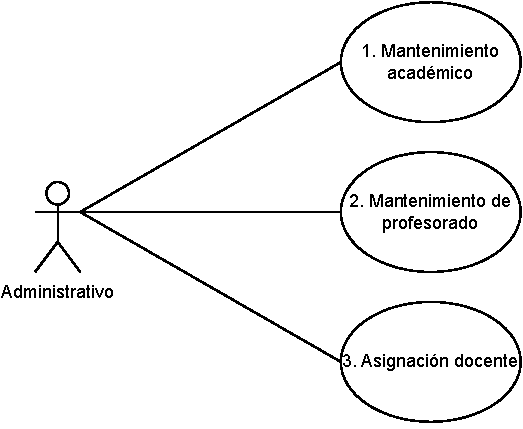
\includegraphics[]{../img/Anexos/Casos uso/Diagrama casos de uso 1.pdf}
	\caption{Diagrama de casos de uso general}
\end{figure}
\FloatBarrier

\begin{table}[p]
	\centering
	\begin{tabularx}{\linewidth}{ p{0.21\columnwidth} p{0.71\columnwidth} }
		\toprule
		\textbf{CU-1}    & \textbf{Mantenimiento docente}\\
		\toprule
		\textbf{Versión}              & 1.0    \\
		\textbf{Autor}                & Ignacio Dávila García \\
		\textbf{Requisitos asociados} & RF-05, RF-01, RF-02 \\
		\textbf{Descripción}          & Un administrativo puede realizar labores de mantenimiento de los centros, titulaciones y asignaturas \\
		\textbf{Precondición}         & Tener iniciada sesión con una cuenta con permisos administrativos \\
		\textbf{Acciones}             &
		\begin{enumerate}
			\def\labelenumi{\arabic{enumi}.}
			\tightlist
			\item Pulsar la opción del menú <<Centros>>, <<Titulaciones>> o <<Asignaturas>>
			\item Se abre la ventana de mantenimiento de la opción elegida.
		\end{enumerate}\\
		\textbf{Postcondición}        & Ninguna \\
		\textbf{Excepciones}          & Según la opción del menú pulsada, la web abre la ventana de mantenimiento de esa opción. Si no se pulsa ninguna, se permanece en la ventana actual. \\
		\textbf{Importancia}          & Alta \\
		\bottomrule
	\end{tabularx}
	\caption{CU-1 Mantenimiento docente.}
\end{table}
\FloatBarrier

\begin{figure}[!h]
	\centering
	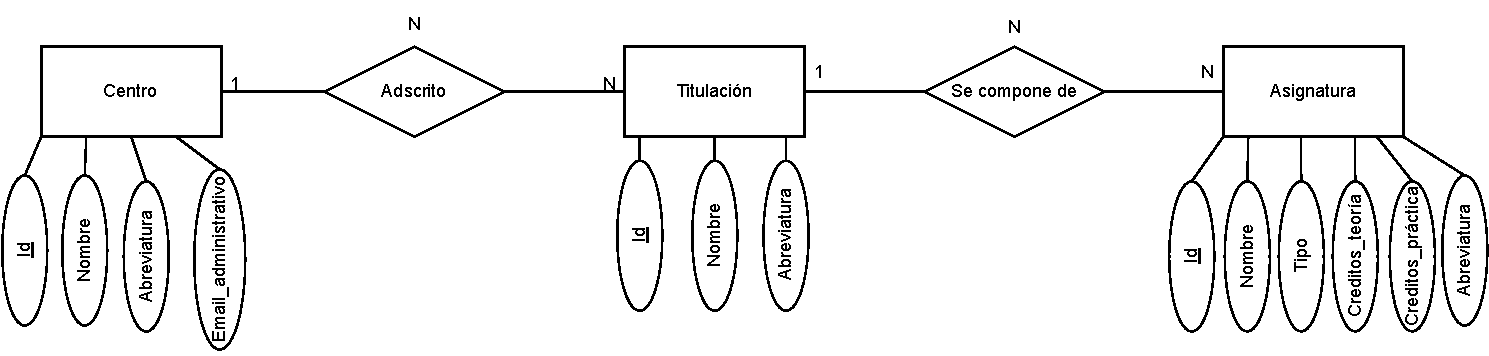
\includegraphics[width=\textwidth]{../img/Anexos/Casos uso/Vistas ER/Diagrama E-R CU 1.pdf}
	\caption{Vista diagrama entidad relación para el CU-1}\label{er_cu1}
\end{figure}
\FloatBarrier

\begin{table}[p]
	\centering
	\begin{tabularx}{\linewidth}{ p{0.21\columnwidth} p{0.71\columnwidth} }
		\toprule
		\textbf{CU-2}    & \textbf{Mantenimiento de profesorado}\\
		\toprule
		\textbf{Versión}              & 1.0    \\
		\textbf{Autor}                & Ignacio Dávila García \\
		\textbf{Requisitos asociados} & RF-04, RF-07, RF-08, RF-09, RF-10 \\
		\textbf{Descripción}          & Un administrativo puede realizar labores de mantenimiento de los docentes, tipos de contrato, departamentos, áreas y plazas. Además, un administrativo puede asignar una plaza a un docente. \\
		\textbf{Precondición}         & Tener iniciada sesión con una cuenta con permisos administrativos \\
		\textbf{Acciones}             &
		\begin{enumerate}
			\def\labelenumi{\arabic{enumi}.}
			\tightlist
			\item Pulsar la opción del menú <<Docentes>>, <<Contratos>>, <<Departamentos>>, <<Áreas>> o <<Plazas>>
			\item Se abre la ventana de mantenimiento de la opción elegida.
		\end{enumerate}\\
		\textbf{Postcondición}        & El sistema lleva al usuario a la ventana de la opción pulsada. \\
		\textbf{Excepciones}          & Ninguna \\
		\textbf{Importancia}          & Alta \\
		\bottomrule
	\end{tabularx}
	\caption{CU-2 Mantenimiento de profesorado.}
\end{table}
\FloatBarrier

\begin{figure}[!h]
	\centering
	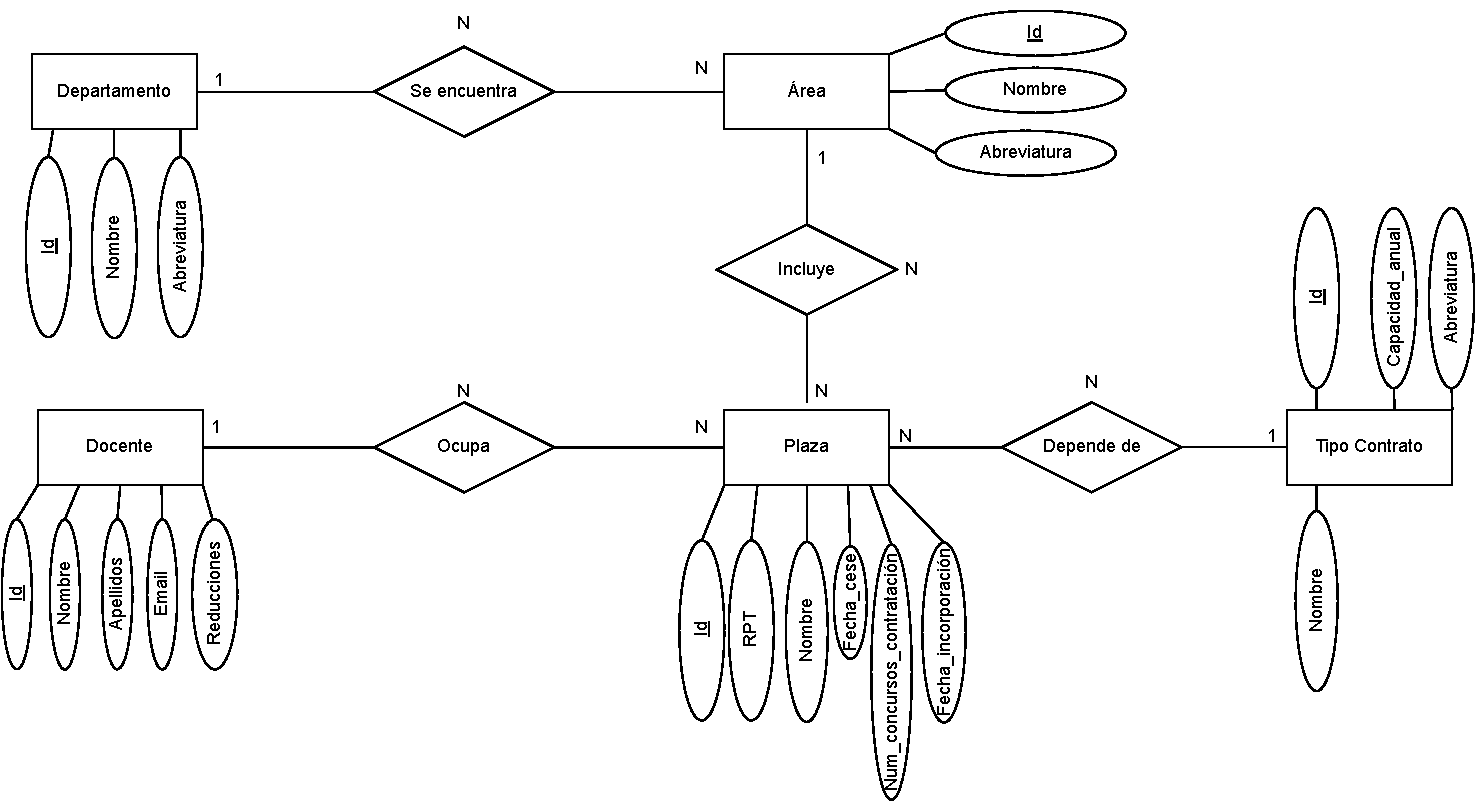
\includegraphics[width=1.2\textwidth]{../img/Anexos/Casos uso/Vistas ER/Diagrama E-R CU 2.pdf}
	\caption{Vista diagrama entidad relación para el CU-2}\label{er_cu2}
\end{figure}
\FloatBarrier

\begin{table}[p]
	\centering
	\begin{tabularx}{\linewidth}{ p{0.21\columnwidth} p{0.71\columnwidth} }
		\toprule
		\textbf{CU-3}    & \textbf{Asignación docente}\\
		\toprule
		\textbf{Versión}              & 1.0    \\
		\textbf{Autor}                & Ignacio Dávila García \\
		\textbf{Requisitos asociados} & RF-04, RF-07, RF-08, RF-09, RF-10 \\
		\textbf{Descripción}          & Un administrativo puede realizar las labores de mantenimiento de cursos y grupos además de las asignaciones de plazas a grupos \\
		\textbf{Precondición}         & Tener iniciada sesión con una cuenta con permisos administrativos \\
		\textbf{Acciones}             &
		\begin{enumerate}
			\def\labelenumi{\arabic{enumi}.}
			\tightlist
			\item Pulsar en la opción del menú <<Cursos>> o <<Grupos>> para realizar los respectivos mantenimientos.
			\item Se abre la ventana de mantenimiento elegida.
			\item Pulsar en la opción <<Horas>> para acceder a la asignación de horas de una plaza a un grupo.
			\item Se abre una ventana que contiene un listado con los diferentes grupos junto a sus plazas/docentes asignados.
		\end{enumerate}\\
		\textbf{Postcondición}        & El sistema lleva al usuario a la ventana de la opción pulsada. \\
		\textbf{Excepciones}          & Ninguna \\
		\textbf{Importancia}          & Alta \\
		\bottomrule
	\end{tabularx}
	\caption{CU-3 Asignación docente.}
\end{table}
\FloatBarrier

\begin{figure}[!h]
	\centering
	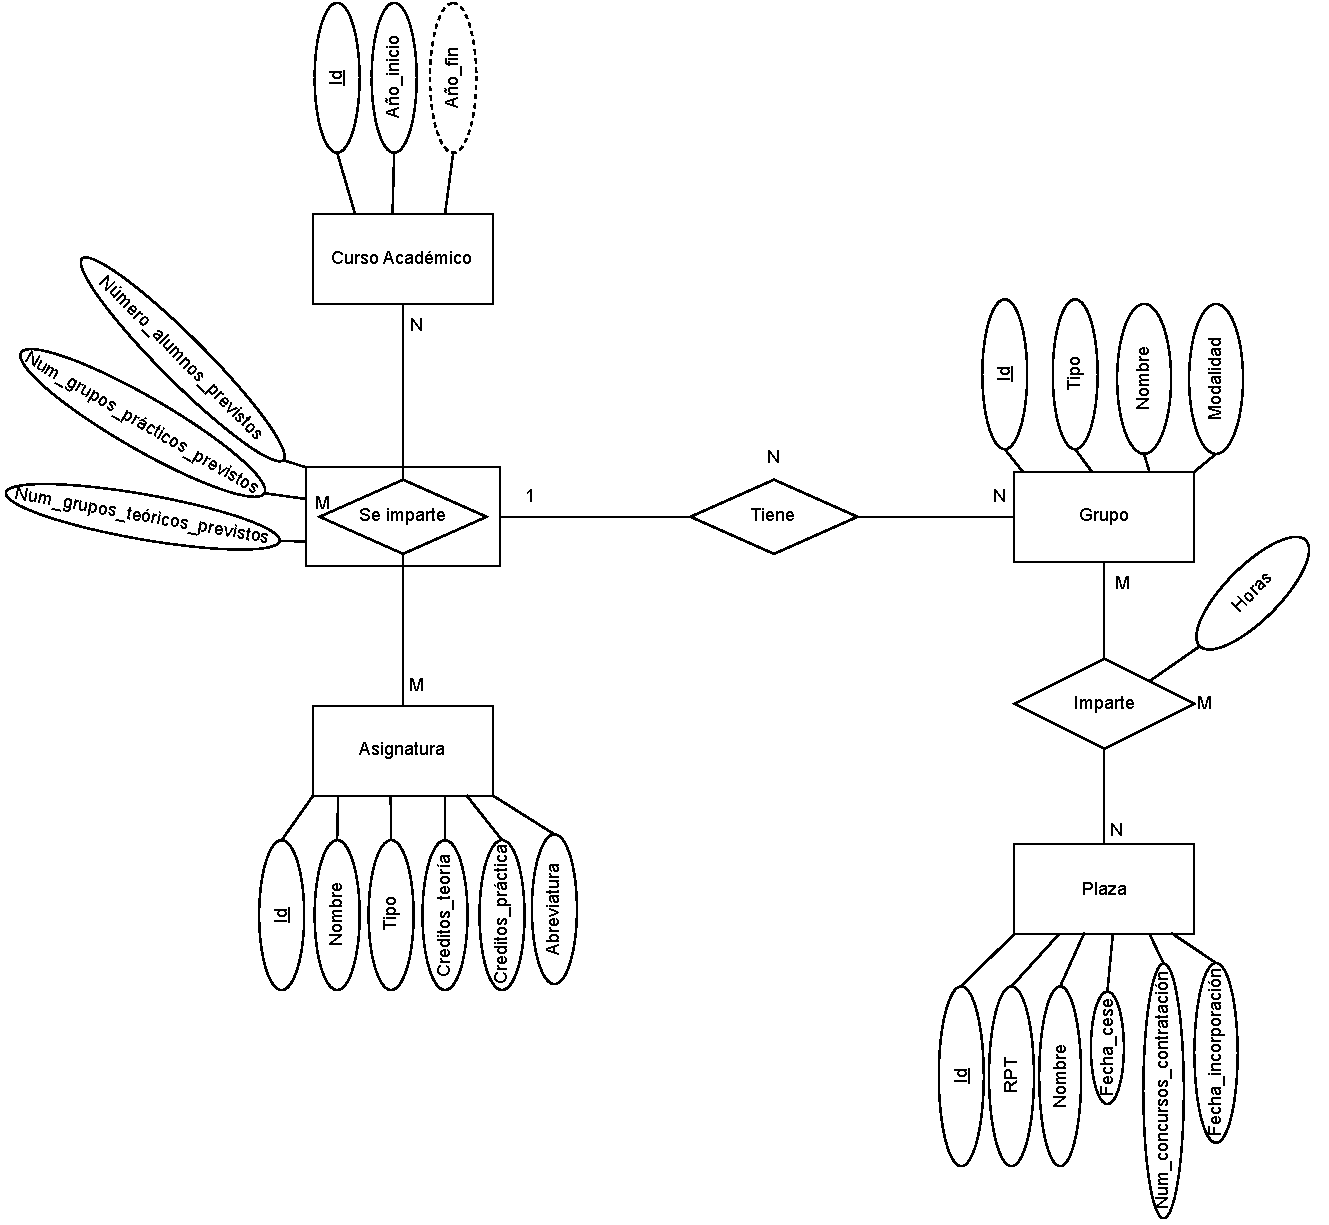
\includegraphics[width=1.2\textwidth]{../img/Anexos/Casos uso/Vistas ER/Diagrama E-R CU 3.pdf}
	\caption{Vista diagrama entidad relación para el CU-3}\label{er_cu3}
\end{figure}
\FloatBarrier

\begin{figure}[!h]
	\centering
	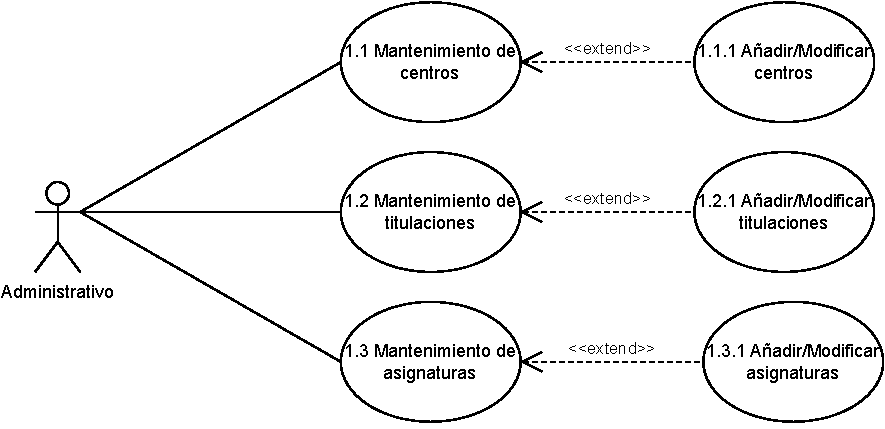
\includegraphics[]{../img/Anexos/Casos uso/Diagrama casos de uso 2.pdf}
	\caption{Diagrama de casos de uso - Mantenimiento docente}
\end{figure}
\FloatBarrier

\begin{table}[p]
	\centering
	\begin{tabularx}{\linewidth}{ p{0.21\columnwidth} p{0.71\columnwidth} }
		\toprule
		\textbf{CU-1.1}    & \textbf{Mantenimiento de centros}\\
		\toprule
		\textbf{Versión}              & 1.0    \\
		\textbf{Autor}                & Ignacio Dávila García \\
		\textbf{Requisitos asociados} & RF-05 \\
		\textbf{Descripción}          & Un administrativo puede realizar el mantenimiento de los centros \\
		\textbf{Precondición}         & Tener iniciada sesión con una cuenta con permisos administrativos \\
		\textbf{Acciones}             &
		\begin{enumerate}
			\def\labelenumi{\arabic{enumi}.}
			\tightlist
			\item Pulsar en la opción <<Centros>> del menú principal de la web.
			\item Se abre una ventana donde aparece una tabla con los centros creados desde donde se podrá realizar el mantenimiento.
		\end{enumerate}\\
		\textbf{Postcondición}        & Ninguna \\
		\textbf{Excepciones}          & Si se pulsa sobre el botón <<Nuevo>>, se accede a la creación de centros. Si se pulsa sobre el botón <<Modificar>> de un centro del listado, se accede a la ventana de <<Modificación>> del centro. Por último, si se pulsa sobre el botón <<Eliminar>> de un centro, este se elimina produciendo un borrado en cascada de las titulaciones vinculadas. \\
		\textbf{Importancia}          & Alta \\
		\bottomrule
	\end{tabularx}
	\caption{CU-1.1 Mantenimiento de centros.}
\end{table}
\FloatBarrier

\begin{table}[p]
	\centering
	\begin{tabularx}{\linewidth}{ p{0.21\columnwidth} p{0.71\columnwidth} }
		\toprule
		\textbf{CU-1.1.1}    & \textbf{Añadir/Modificar centros}\\
		\toprule
		\textbf{Versión}              & 1.0    \\
		\textbf{Autor}                & Ignacio Dávila García \\
		\textbf{Requisitos asociados} & RF-05 \\
		\textbf{Descripción}          & Un administrativo añade o modifica un nuevo centro \\
		\textbf{Precondición}         & Tener iniciada sesión con una cuenta con permisos administrativos \\
		\textbf{Acciones}             &
		\begin{enumerate}
			\def\labelenumi{\arabic{enumi}.}
			\tightlist
			\item Pulsar en la opción <<Centros>> del menú principal de la web.
			\item Se abre una ventana donde aparece una tabla con los centros creados.
			\item Pulsar sobre el botón <<Nuevo>> para añadir un nuevo centro.
			\item Se abre una nueva ventana con un formulario vacío donde aparecen los campos de la tabla <<Centro>> de la figura \ref{er_cu1}, necesarios para crear un centro).
			\item Rellenar el formulario con los datos del centro que se desea añadir.
			\item Pulsar sobre el botón <<Añadir>>.
		\end{enumerate}\\
		\textbf{Postcondición}        & El centro queda añadido/modificado y el sistema lleva al usuario a la ventana de centros donde se puede ver el listado de todos los centros creados. \\
		\textbf{Excepciones}          & Se dejan campos vacíos o se introducen datos con un formato incorrecto. Otra forma de finalizar el caso de uso es la modificación. En este caso, se pulsa sobre el botón <<Modificar>> de un centro y se accede al mismo formulario con los campos rellenos. Finalmente se pulsa en el botón <<Modificar>> \\
		\textbf{Importancia}          & Alta \\
		\bottomrule
	\end{tabularx}
	\caption{CU-1.1.1 Añadir/Modificar centros.}
\end{table}
\FloatBarrier

\begin{table}[p]
	\centering
	\begin{tabularx}{\linewidth}{ p{0.21\columnwidth} p{0.71\columnwidth} }
		\toprule
		\textbf{CU-1.2}    & \textbf{Mantenimiento de titulaciones}\\
		\toprule
		\textbf{Versión}              & 1.0    \\
		\textbf{Autor}                & Ignacio Dávila García \\
		\textbf{Requisitos asociados} & RF-01 \\
		\textbf{Descripción}          & Un administrativo puede realizar el mantenimiento de las titulaciones \\
		\textbf{Precondición}         & Tener iniciada sesión con una cuenta con permisos administrativos \\
		\textbf{Acciones}             &
		\begin{enumerate}
			\def\labelenumi{\arabic{enumi}.}
			\tightlist
			\item Pulsar en la opción <<Titulaciones>> del menú principal de la web.
			\item Se abre una ventana donde aparece una tabla con las titulaciones creadas desde donde se podrá realizar el mantenimiento.
		\end{enumerate}\\
		\textbf{Postcondición}        & Ninguna \\
		\textbf{Excepciones}          & Si se pulsa sobre el botón <<Nuevo>>, se accede a la creación de titulaciones. Si se pulsa sobre el botón <<Modificar>> de una titulación de la lista, se accede a la ventana de modificación. Por último, si se pulsa sobre el botón <<Eliminar>> de una titulación, esta se elimina produciendo un borrado en cascada de las asignaturas vinculadas. \\
		\textbf{Importancia}          & Alta \\
		\bottomrule
	\end{tabularx}
	\caption{CU-1.2 Mantenimiento de titulaciones.}
\end{table}
\FloatBarrier

\begin{table}[p]
	\centering
	\begin{tabularx}{\linewidth}{ p{0.21\columnwidth} p{0.71\columnwidth} }
		\toprule
		\textbf{CU-1.2.1}    & \textbf{Añadir/Modificar titulaciones}\\
		\toprule
		\textbf{Versión}              & 1.0    \\
		\textbf{Autor}                & Ignacio Dávila García \\
		\textbf{Requisitos asociados} & RF-01 \\
		\textbf{Descripción}          & Un administrativo añade o modifica una titulación \\
		\textbf{Precondición}         & Tener iniciada sesión con una cuenta con permisos administrativos y tener algún centro creado \\
		\textbf{Acciones}             &
		\begin{enumerate}
			\def\labelenumi{\arabic{enumi}.}
			\tightlist
			\item Pulsar en la opción <<Titulaciones>> del menú principal de la web.
			\item Se abre una ventana donde aparece una tabla con todas las titulaciones.
			\item Pulsar sobre el botón <<Nuevo>> para añadir una nueva titulación.
			\item Se abre una nueva ventana con un formulario vacío donde aparecen los campos de la tabla <<Titulación>> de la figura \ref{er_cu1}, necesarios para crear una titulación.
			\item Rellenar el formulario con los datos de la titulación que se desea añadir.
			\item Pulsar sobre el botón <<Añadir>>.
		\end{enumerate}\\
		\textbf{Postcondición}        & La titulación queda añadida/modificada y el sistema lleva al usuario a la ventana de titulaciones donde se puede ver el listado de todos las titulaciones añadidas. \\
		\textbf{Excepciones}          & Se dejan campos vacíos o se introducen datos con un formato incorrecto. Otra forma de finalizar el caso de uso es la modificación. En este caso, se pulsa sobre el botón <<Modificar>> de una titulación de la tabla y se accede al mismo formulario, pero con los campos rellenos. Finalmente se pulsa en el botón <<Modificar>> y la titulación queda modificada. \\
		\textbf{Importancia}          & Alta \\
		\bottomrule
	\end{tabularx}
	\caption{CU-1.2.1 Añadir/Modificar centros.}
\end{table}
\FloatBarrier

\begin{table}[p]
	\centering
	\begin{tabularx}{\linewidth}{ p{0.21\columnwidth} p{0.71\columnwidth} }
		\toprule
		\textbf{CU-1.3}    & \textbf{Mantenimiento de asignaturas}\\
		\toprule
		\textbf{Versión}              & 1.0    \\
		\textbf{Autor}                & Ignacio Dávila García \\
		\textbf{Requisitos asociados} & RF-02 \\
		\textbf{Descripción}          & Un administrativo puede realizar el mantenimiento de asignaturas \\
		\textbf{Precondición}         & Tener iniciada sesión con una cuenta con permisos administrativos \\
		\textbf{Acciones}             &
		\begin{enumerate}
			\def\labelenumi{\arabic{enumi}.}
			\tightlist
			\item Pulsar en la opción <<Asignaturas>> del menú principal de la web.
			\item Se abre una ventana donde aparece una tabla con las asignaturas creadas desde donde se podrá realizar el mantenimiento.
		\end{enumerate}\\
		\textbf{Postcondición}        & Ninguna \\
		\textbf{Excepciones}          & Si se pulsa sobre el botón <<Nuevo>>, se accede a la creación de asignaturas. Si se pulsa sobre el botón <<Modificar>> de una asignaturas de la lista, se accede a la ventana de modificación. Por último, si se pulsa sobre el botón <<Eliminar>> de una asignaturas, esta se elimina. \\
		\textbf{Importancia}          & Alta \\
		\bottomrule
	\end{tabularx}
	\caption{CU-1.3 Mantenimiento de asignaturas.}
\end{table}
\FloatBarrier

\begin{table}[p]
	\centering
	\begin{tabularx}{\linewidth}{ p{0.21\columnwidth} p{0.71\columnwidth} }
		\toprule
		\textbf{CU-1.3.1}    & \textbf{Añadir/Modificar asignaturas}\\
		\toprule
		\textbf{Versión}              & 1.0    \\
		\textbf{Autor}                & Ignacio Dávila García \\
		\textbf{Requisitos asociados} & RF-02 \\
		\textbf{Descripción}          & Un administrativo añade o modifica una asignatura \\
		\textbf{Precondición}         & Tener iniciada sesión con una cuenta con permisos administrativos y tener alguna titulación creada \\
		\textbf{Acciones}             &
		\begin{enumerate}
			\def\labelenumi{\arabic{enumi}.}
			\tightlist
			\item Pulsar en la opción <<Asignaturas>> del menú principal de la web.
			\item Se abre una ventana donde aparece una tabla con todas las asignaturas.
			\item Pulsar sobre el botón <<Nuevo>> para añadir una nueva asignatura.
			\item Se abre una nueva ventana con un formulario vacío donde aparecen los campos de la tabla <<Asignatura>> de la figura \ref{er_cu1}, necesarios para crear una asignatura.
			\item Rellenar el formulario con los datos de la asignatura que se desea añadir.
			\item Pulsar sobre el botón <<Añadir>>.
		\end{enumerate}\\
		\textbf{Postcondición}        & La asignatura queda añadida/modificada y el sistema lleva al usuario a la ventana de asignaturas donde se puede ver el listado de todos las asignaturas añadidas. \\
		\textbf{Excepciones}          & Se dejan campos vacíos o se introducen datos con un formato incorrecto. Otra forma de finalizar el caso de uso es la modificación. En este caso, se pulsa sobre el botón <<Modificar>> de una asignatura de la tabla y se accede al mismo formulario, pero con los campos rellenos. Finalmente se pulsa en el botón <<Modificar>> y la asignatura queda modificada. \\
		\textbf{Importancia}          & Alta \\
		\bottomrule
	\end{tabularx}
	\caption{CU-1.3.1 Añadir/Modificar asignaturas.}
\end{table}
\FloatBarrier

\begin{figure}[!h]
	\centering
	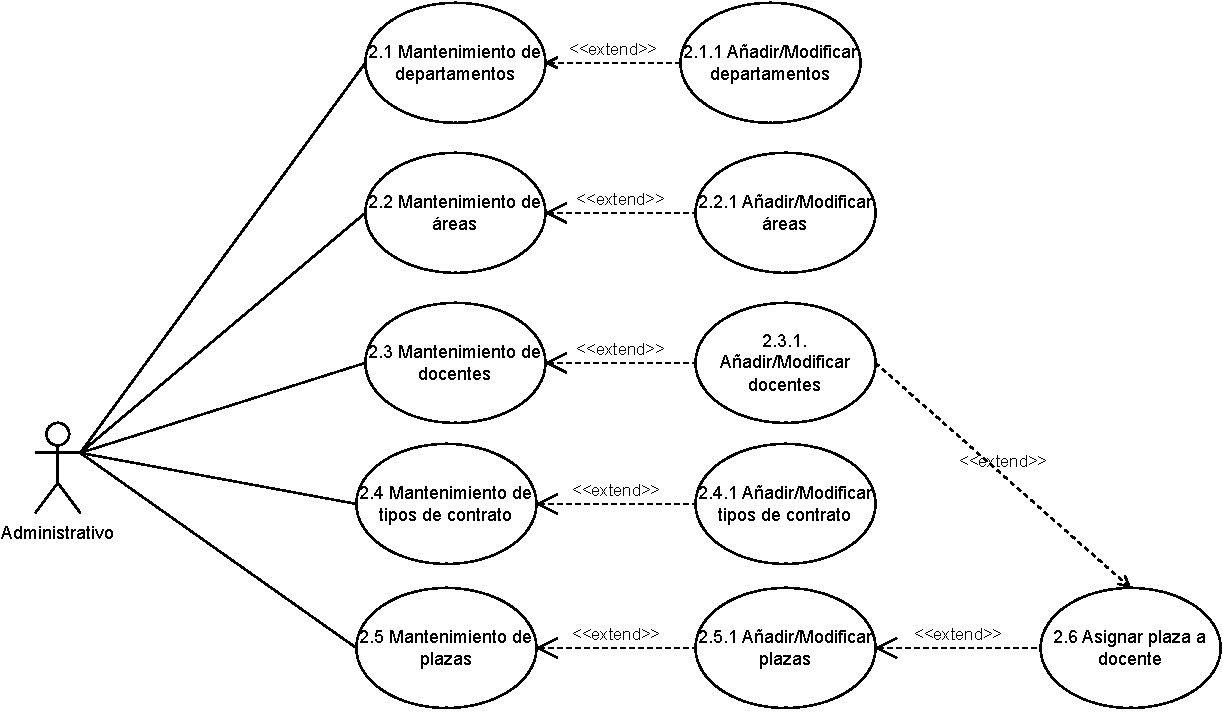
\includegraphics[width=1.1\textwidth]{../img/Anexos/Casos uso/Diagrama casos de uso 3.pdf}
	\caption{Diagrama de casos de uso - Mantenimiento de profesorado}
\end{figure}
\FloatBarrier

\begin{table}[p]
	\centering
	\begin{tabularx}{\linewidth}{ p{0.21\columnwidth} p{0.71\columnwidth} }
		\toprule
		\textbf{CU-2.1}    & \textbf{Mantenimiento de departamentos}\\
		\toprule
		\textbf{Versión}              & 1.0    \\
		\textbf{Autor}                & Ignacio Dávila García \\
		\textbf{Requisitos asociados} & RF-10 \\
		\textbf{Descripción}          & Un administrativo puede realizar el mantenimiento de departamentos \\
		\textbf{Precondición}         & Tener iniciada sesión con una cuenta con permisos administrativos \\
		\textbf{Acciones}             &
		\begin{enumerate}
			\def\labelenumi{\arabic{enumi}.}
			\tightlist
			\item Pulsar en la opción <<Departamentos>> del menú principal de la web.
			\item Se abre una ventana donde aparece una tabla con los departamentos creados desde donde se podrá realizar el mantenimiento.
		\end{enumerate}\\
		\textbf{Postcondición}        & Ninguna \\
		\textbf{Excepciones}          & Si se pulsa sobre el botón <<Nuevo>>, se accede a la creación de departamentos. Si se pulsa sobre el botón <<Modificar>> de un departamento de la lista, se accede a la ventana de modificación. Por último, si se pulsa sobre el botón <<Eliminar>> de un departamento, este se elimina produciendo un borrado en cascada de las áreas asociadas. \\
		\textbf{Importancia}          & Alta \\
		\bottomrule
	\end{tabularx}
	\caption{CU-2.1 Mantenimiento de departamentos.}
\end{table}
\FloatBarrier

\begin{table}[p]
	\centering
	\begin{tabularx}{\linewidth}{ p{0.21\columnwidth} p{0.71\columnwidth} }
		\toprule
		\textbf{CU-2.1.1}    & \textbf{Añadir/Modificar departamentos}\\
		\toprule
		\textbf{Versión}              & 1.0    \\
		\textbf{Autor}                & Ignacio Dávila García \\
		\textbf{Requisitos asociados} & RF-10 \\
		\textbf{Descripción}          & Un administrativo añade o modifica un departamento \\
		\textbf{Precondición}         & Tener iniciada sesión con una cuenta con permisos administrativos \\
		\textbf{Acciones}             &
		\begin{enumerate}
			\def\labelenumi{\arabic{enumi}.}
			\tightlist
			\item Pulsar en la opción <<Departamentos>> del menú principal de la web.
			\item Se abre una ventana donde aparece una tabla con todos los departamentos.
			\item Pulsar sobre el botón <<Nuevo>> para añadir un nuevo departamento.
			\item Se abre una nueva ventana con un formulario vacío donde aparecen los campos de la tabla <<Departamento>> de la figura \ref{er_cu2}, necesarios para crear un departamento.
			\item Rellenar el formulario con los datos del departamento que se desea añadir.
			\item Pulsar sobre el botón <<Añadir>>.
		\end{enumerate}\\
		\textbf{Postcondición}        & El departamento queda añadido/modificado y el sistema lleva al usuario a la ventana de departamentos donde se puede ver el listado de todos los departamento añadidos. \\
		\textbf{Excepciones}          & Se dejan campos vacíos o se introducen datos con un formato incorrecto. Otra forma de finalizar el caso de uso es la modificación. En este caso, se pulsa sobre el botón <<Modificar>> de un departamento de la tabla y se accede al mismo formulario, pero con los campos rellenos. Finalmente se pulsa en el botón <<Modificar>> y el departamento queda modificado. \\
		\textbf{Importancia}          & Alta \\
		\bottomrule
	\end{tabularx}
	\caption{CU-2.1.1 Añadir/Modificar departamentos.}
\end{table}
\FloatBarrier

\begin{table}[p]
	\centering
	\begin{tabularx}{\linewidth}{ p{0.21\columnwidth} p{0.71\columnwidth} }
		\toprule
		\textbf{CU-2.2}    & \textbf{Mantenimiento de áreas}\\
		\toprule
		\textbf{Versión}              & 1.0    \\
		\textbf{Autor}                & Ignacio Dávila García \\
		\textbf{Requisitos asociados} & RF-09 \\
		\textbf{Descripción}          & Un administrativo puede realizar el mantenimiento de áreas \\
		\textbf{Precondición}         & Tener iniciada sesión con una cuenta con permisos administrativos \\
		\textbf{Acciones}             &
		\begin{enumerate}
			\def\labelenumi{\arabic{enumi}.}
			\tightlist
			\item Pulsar en la opción <<Áreas>> del menú principal de la web.
			\item Se abre una ventana donde aparece una tabla con las áreas creadas desde donde se podrá realizar el mantenimiento.
		\end{enumerate}\\
		\textbf{Postcondición}        & Ninguna \\
		\textbf{Excepciones}          & Si se pulsa sobre el botón <<Nuevo>>, se accede a la creación de áreas. Si se pulsa sobre el botón <<Modificar>> de un área de la lista, se accede a la ventana de modificación. Por último, si se pulsa sobre el botón <<Eliminar>> de un área, esta se elimina produciendo un borrado en cascada de las plazas asociadas. \\
		\textbf{Importancia}          & Alta \\
		\bottomrule
	\end{tabularx}
	\caption{CU-2.2 Mantenimiento de áreas.}
\end{table}
\FloatBarrier

\begin{table}[p]
	\centering
	\begin{tabularx}{\linewidth}{ p{0.21\columnwidth} p{0.71\columnwidth} }
		\toprule
		\textbf{CU-2.2.1}    & \textbf{Añadir/Modificar áreas}\\
		\toprule
		\textbf{Versión}              & 1.0    \\
		\textbf{Autor}                & Ignacio Dávila García \\
		\textbf{Requisitos asociados} & RF-09 \\
		\textbf{Descripción}          & Un administrativo añade o modifica un área \\
		\textbf{Precondición}         & Tener iniciada sesión con una cuenta con permisos administrativos y tener algún departamento creado \\
		\textbf{Acciones}             &
		\begin{enumerate}
			\def\labelenumi{\arabic{enumi}.}
			\tightlist
			\item Pulsar en la opción <<Áreas>> del menú principal de la web.
			\item Se abre una ventana donde aparece una tabla con todas las áreas.
			\item Pulsar sobre el botón <<Nuevo>> para añadir un nuevo área.
			\item Se abre una nueva ventana con un formulario vacío donde aparecen los campos de la tabla <<Área>> de la figura \ref{er_cu2}, necesarios para crear un área.
			\item Rellenar el formulario con los datos del área que se desea añadir.
			\item Pulsar sobre el botón <<Añadir>>.
		\end{enumerate}\\
		\textbf{Postcondición}        & El área queda añadido/modificado y el sistema lleva al usuario a la ventana de áreas donde se puede ver el listado de todas las áreas añadidas. \\
		\textbf{Excepciones}          & Se dejan campos vacíos o se introducen datos con un formato incorrecto. Otra forma de finalizar el caso de uso es la modificación. En este caso, se pulsa sobre el botón <<Modificar>> de un área de la tabla y se accede al mismo formulario, pero con los campos rellenos. Finalmente se pulsa en el botón <<Modificar>> y el área queda modificado. \\
		\textbf{Importancia}          & Alta \\
		\bottomrule
	\end{tabularx}
	\caption{CU-2.2.1 Añadir/Modificar áreas.}
\end{table}
\FloatBarrier

\begin{table}[p]
	\centering
	\begin{tabularx}{\linewidth}{ p{0.21\columnwidth} p{0.71\columnwidth} }
		\toprule
		\textbf{CU-2.3}    & \textbf{Mantenimiento de docentes}\\
		\toprule
		\textbf{Versión}              & 1.0    \\
		\textbf{Autor}                & Ignacio Dávila García \\
		\textbf{Requisitos asociados} & RF-04 \\
		\textbf{Descripción}          & Un administrativo puede realizar el mantenimiento de docentes \\
		\textbf{Precondición}         & Tener iniciada sesión con una cuenta con permisos administrativos \\
		\textbf{Acciones}             &
		\begin{enumerate}
			\def\labelenumi{\arabic{enumi}.}
			\tightlist
			\item Pulsar en la opción <<Docentes>> del menú principal de la web.
			\item Se abre una ventana donde aparece una tabla con los docentes creados desde donde se podrá realizar el mantenimiento.
		\end{enumerate}\\
		\textbf{Postcondición}        & Ninguna \\
		\textbf{Excepciones}          & Si se pulsa sobre el botón <<Nuevo>>, se accede a la creación de docentes. Si se pulsa sobre el botón <<Modificar>> de un docente de la lista, se accede a la ventana de modificación. Por último, si se pulsa sobre el botón <<Eliminar>> de un docente, este se elimina. \\
		\textbf{Importancia}          & Alta \\
		\bottomrule
	\end{tabularx}
	\caption{CU-2.3 Mantenimiento de docentes.}
\end{table}
\FloatBarrier

\begin{table}[p]
	\centering
	\begin{tabularx}{\linewidth}{ p{0.21\columnwidth} p{0.71\columnwidth} }
		\toprule
		\textbf{CU-2.3.1}    & \textbf{Añadir/Modificar docentes}\\
		\toprule
		\textbf{Versión}              & 1.0    \\
		\textbf{Autor}                & Ignacio Dávila García \\
		\textbf{Requisitos asociados} & RF-04 \\
		\textbf{Descripción}          & Un administrativo añade o modifica un docente \\
		\textbf{Precondición}         & Tener iniciada sesión con una cuenta con permisos administrativos \\
		\textbf{Acciones}             &
		\begin{enumerate}
			\def\labelenumi{\arabic{enumi}.}
			\tightlist
			\item Pulsar en la opción <<Docentes>> del menú principal de la web.
			\item Se abre una ventana donde aparece una tabla con todos los docentes existentes.
			\item Pulsar sobre el botón <<Nuevo>> para añadir un nuevo docente.
			\item Se abre una nueva ventana con un formulario vacío donde aparecen los campos de la tabla <<Docente>> de la figura \ref{er_cu2}, necesarios para crear un docente.
			\item Rellenar el formulario con los datos del docente que se desea añadir.
			\item Pulsar sobre el botón <<Añadir>>.
		\end{enumerate}\\
		\textbf{Postcondición}        & El docente queda añadido/modificado y el sistema lleva al usuario a la ventana de docentes donde se puede ver el listado de todos los docentes añadidos. \\
		\textbf{Excepciones}          & Se dejan campos vacíos o se introducen datos con un formato incorrecto. Otra forma de finalizar el caso de uso es la modificación. En este caso, se pulsa sobre el botón <<Modificar>> de un docente de la tabla y se accede al mismo formulario, pero con los campos rellenos. Finalmente se pulsa en el botón <<Modificar>> y el docente queda modificado. \\
		\textbf{Importancia}          & Alta \\
		\bottomrule
	\end{tabularx}
	\caption{CU-2.3.1 Añadir/Modificar docentes.}
\end{table}
\FloatBarrier

\begin{table}[p]
	\centering
	\begin{tabularx}{\linewidth}{ p{0.21\columnwidth} p{0.71\columnwidth} }
		\toprule
		\textbf{CU-2.4}    & \textbf{Mantenimiento de tipos de contrato}\\
		\toprule
		\textbf{Versión}              & 1.0    \\
		\textbf{Autor}                & Ignacio Dávila García \\
		\textbf{Requisitos asociados} & RF-08 \\
		\textbf{Descripción}          & Un administrativo puede realizar el mantenimiento de tipos de contrato \\
		\textbf{Precondición}         & Tener iniciada sesión con una cuenta con permisos administrativos \\
		\textbf{Acciones}             &
		\begin{enumerate}
			\def\labelenumi{\arabic{enumi}.}
			\tightlist
			\item Pulsar en la opción <<Contratos>> del menú principal de la web.
			\item Se abre una ventana donde aparece una tabla con los tipos de contrato creados desde donde se podrá realizar el mantenimiento.
		\end{enumerate}\\
		\textbf{Postcondición}        & Ninguna \\
		\textbf{Excepciones}          & Si se pulsa sobre el botón <<Nuevo>>, se accede a la creación de un nuevo tipo de contrato. Si se pulsa sobre el botón <<Modificar>> de un tipo de contrato de la lista, se accede a la ventana de modificación. Por último, si se pulsa sobre el botón <<Eliminar>> de un tipo de contrato, este se elimina. \\
		\textbf{Importancia}          & Alta \\
		\bottomrule
	\end{tabularx}
	\caption{CU-2.4 Mantenimiento de tipos de contrato.}
\end{table}
\FloatBarrier

\begin{table}[p]
	\centering
	\begin{tabularx}{\linewidth}{ p{0.21\columnwidth} p{0.71\columnwidth} }
		\toprule
		\textbf{CU-2.4.1}    & \textbf{Añadir/Modificar tipos de contrato}\\
		\toprule
		\textbf{Versión}              & 1.0    \\
		\textbf{Autor}                & Ignacio Dávila García \\
		\textbf{Requisitos asociados} & RF-08 \\
		\textbf{Descripción}          & Un administrativo añade o modifica un docente \\
		\textbf{Precondición}         & Tener iniciada sesión con una cuenta con permisos administrativos \\
		\textbf{Acciones}             &
		\begin{enumerate}
			\def\labelenumi{\arabic{enumi}.}
			\tightlist
			\item Pulsar en la opción <<Contratos>> del menú principal de la web.
			\item Se abre una ventana donde aparece una tabla con todos los tipos de contrato existentes.
			\item Pulsar sobre el botón <<Nuevo>> para añadir un nuevo tipo de contrato.
			\item Se abre una nueva ventana con un formulario vacío donde aparecen los campos de la tabla <<Tipo Contrato>> de la figura \ref{er_cu2}, necesarios para crear un tipo de contrato.
			\item Rellenar el formulario con los datos del tipo de contrato que se desea añadir.
			\item Pulsar sobre el botón <<Añadir>>.
		\end{enumerate}\\
		\textbf{Postcondición}        & El tipo de contrato queda añadido/modificado y el sistema lleva al usuario a la ventana de tipos de contrato donde se puede ver el listado de todos los tipos de contrato añadidos. \\
		\textbf{Excepciones}          & Se dejan campos vacíos o se introducen datos con un formato incorrecto. Otra forma de finalizar el caso de uso es la modificación. En este caso, se pulsa sobre el botón <<Modificar>> de un tipo de contrato de la tabla y se accede al mismo formulario, pero con los campos rellenos. Finalmente se pulsa en el botón <<Modificar>> y el tipo de contrato queda modificado. \\
		\textbf{Importancia}          & Alta \\
		\bottomrule
	\end{tabularx}
	\caption{CU-2.4.1 Añadir/Modificar tipos de contrato.}
\end{table}
\FloatBarrier

\begin{table}[p]
	\centering
	\begin{tabularx}{\linewidth}{ p{0.21\columnwidth} p{0.71\columnwidth} }
		\toprule
		\textbf{CU-2.5}    & \textbf{Mantenimiento de plazas}\\
		\toprule
		\textbf{Versión}              & 1.0    \\
		\textbf{Autor}                & Ignacio Dávila García \\
		\textbf{Requisitos asociados} & RF-07 \\
		\textbf{Descripción}          & Un administrativo puede realizar el mantenimiento de plazas \\
		\textbf{Precondición}         & Tener iniciada sesión con una cuenta con permisos administrativos \\
		\textbf{Acciones}             &
		\begin{enumerate}
			\def\labelenumi{\arabic{enumi}.}
			\tightlist
			\item Pulsar en la opción <<Plazas>> del menú principal de la web.
			\item Se abre una ventana donde aparece una tabla con las plazas creadas desde donde se podrá realizar el mantenimiento.
		\end{enumerate}\\
		\textbf{Postcondición}        & Ninguna \\
		\textbf{Excepciones}          & Si se pulsa sobre el botón <<Nuevo>>, se accede a la creación de una plaza. Si se pulsa sobre el botón <<Modificar>> de una plaza de la lista, se accede a la ventana de modificación. Por último, si se pulsa sobre el botón <<Eliminar>> de una plaza, este se elimina. \\
		\textbf{Importancia}          & Alta \\
		\bottomrule
	\end{tabularx}
	\caption{CU-2.5 Mantenimiento de plazas.}
\end{table}
\FloatBarrier

\begin{table}[p]
	\centering
	\begin{tabularx}{\linewidth}{ p{0.21\columnwidth} p{0.71\columnwidth} }
		\toprule
		\textbf{CU-2.5.1}    & \textbf{Añadir/Modificar plazas}\\
		\toprule
		\textbf{Versión}              & 1.0    \\
		\textbf{Autor}                & Ignacio Dávila García \\
		\textbf{Requisitos asociados} & RF-07 \\
		\textbf{Descripción}          & Un administrativo añade o modifica una plaza \\
		\textbf{Precondición}         & Tener iniciada sesión con una cuenta con permisos administrativos y tener algún área y tipo de contrato creados \\
		\textbf{Acciones}             &
		\begin{enumerate}
			\def\labelenumi{\arabic{enumi}.}
			\tightlist
			\item Pulsar en la opción <<Plazas>> del menú principal de la web.
			\item Se abre una ventana donde aparece una tabla con todas las plazas existentes.
			\item Pulsar sobre el botón <<Nuevo>> para añadir una nueva plaza.
			\item Se abre una nueva ventana con un formulario vacío donde aparecen los campos de la tabla <<Plaza>> de la figura \ref{er_cu2}, necesarios para crear una plaza.
			\item Rellenar el formulario con los datos de la plaza que se desea añadir.
			\item Pulsar sobre el botón <<Añadir>>.
		\end{enumerate}\\
		\textbf{Postcondición}        & La plaza queda añadida/modificada y el sistema lleva al usuario a la ventana de plazas donde se puede ver el listado de todas las plazas añadidas. \\
		\textbf{Excepciones}          & Se dejan campos vacíos o se introducen datos con un formato incorrecto. Otra forma de finalizar el caso de uso es la modificación. En este caso, se pulsa sobre el botón <<Modificar>> de una plaza de la tabla y se accede al mismo formulario, pero con los campos rellenos. Finalmente se pulsa en el botón <<Modificar>> y la plaza queda modificada. \\
		\textbf{Importancia}          & Alta \\
		\bottomrule
	\end{tabularx}
	\caption{CU-2.5.1 Añadir/Modificar plazas.}
\end{table}
\FloatBarrier

\begin{table}[p]
	\centering
	\begin{tabularx}{\linewidth}{ p{0.21\columnwidth} p{0.71\columnwidth} }
		\toprule
		\textbf{CU-2.6}    & \textbf{Asignar plaza a docente}\\
		\toprule
		\textbf{Versión}              & 1.0    \\
		\textbf{Autor}                & Ignacio Dávila García \\
		\textbf{Requisitos asociados} & RF-07, RF-12 \\
		\textbf{Descripción}          & Un administrativo puede asignar una plaza a un docente. Este caso de uso es una extensión del CU-2.5.1, ya que la asignación de la plaza a un docente se realiza en la creación o modificación de la misma \\
		\textbf{Precondición}         & Tener iniciada sesión con una cuenta con permisos administrativos y tener creado un docente \\
		\textbf{Acciones}             &
		\begin{enumerate}
			\def\labelenumi{\arabic{enumi}.}
			\tightlist
			\item Pulsar en la opción <<Plazas>> del menú principal de la web.
			\item Se abre una ventana donde aparece una tabla con las plazas creadas.
			\item Si la plaza que se desea asignar ya está creada, pulsar en el botón <<Modificar>> de la fila de la tabla que corresponde a la plaza.
			\item Si la plaza todavía no está creada, pulsar en el botón <<Nuevo>>
			\item Se abre una ventana con un formulario que tendrá los campos de la tabla <<Plaza>> de la figura \ref{er_cu2} vacíos si es una creación o los campos rellenos si es una modificación. En el campo llamado <<Docente>>, se podrá seleccionar el docente al que se quiere asignar la plaza desde un seleccionable con búsqueda.
		\end{enumerate}\\
		\textbf{Postcondición}        & Ninguna \\
		\textbf{Excepciones}          & Si se pulsa sobre el botón <<Añadir>>, en el caso de una creación, la plaza queda añadida y el sistema lleva al usuario a la ventana del mantenimiento de plazas. En el caso de una modificación, si se pulsa sobre el botón <<Modificar>>, la plaza queda modificada y asignada al docente seleccionado y el sistema lleva al usuario a la ventana de mantenimiento de plazas. \\
		\textbf{Importancia}          & Alta \\
		\bottomrule
	\end{tabularx}
	\caption{CU-2.6 Asignar plaza a docente.}
\end{table}
\FloatBarrier

\begin{figure}[!h]
	\centering
	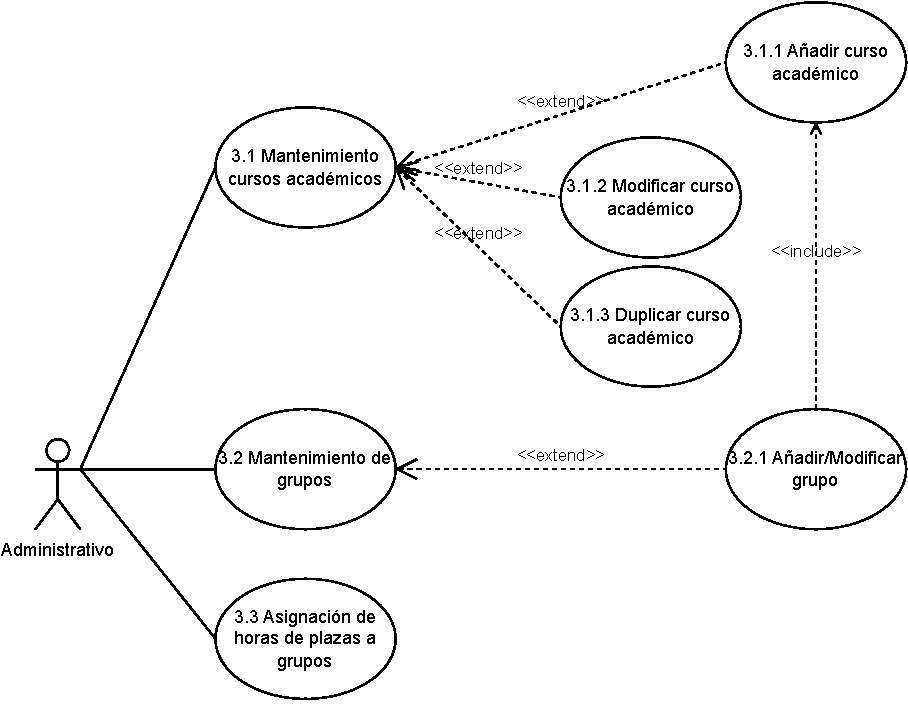
\includegraphics[]{../img/Anexos/Casos uso/Diagrama casos de uso 4.pdf}
	\caption{Diagrama de casos de uso - Asignación docente}
\end{figure}
\FloatBarrier

\begin{table}[p]
	\centering
	\begin{tabularx}{\linewidth}{ p{0.21\columnwidth} p{0.71\columnwidth} }
		\toprule
		\textbf{CU-3.1}    & \textbf{Mantenimiento cursos académicos}\\
		\toprule
		\textbf{Versión}              & 1.0    \\
		\textbf{Autor}                & Ignacio Dávila García \\
		\textbf{Requisitos asociados} & RF-06 \\
		\textbf{Descripción}          & Un administrativo puede realizar el mantenimiento de los cursos académicos \\
		\textbf{Precondición}         & Tener iniciada sesión con una cuenta con permisos administrativos \\
		\textbf{Acciones}             &
		\begin{enumerate}
			\def\labelenumi{\arabic{enumi}.}
			\tightlist
			\item Pulsar en la opción <<Cursos>> del menú principal de la web.
			\item Se abre una ventana donde aparece una tabla con los cursos creados desde donde se podrá realizar el mantenimiento.
		\end{enumerate}\\
		\textbf{Postcondición}        & Ninguna \\
		\textbf{Excepciones}          & Si se pulsa sobre el botón <<Nuevo>>, se accede a la creación de un curso. Si se pulsa sobre el botón <<Modificar>> de un curso de la lista, se accede a la ventana de modificación. Si se pulsa sobre el botón <<Modificar Año>> de un curso de la lista, se accede a la ventana de modificación del campo año de inicio. Por último, si se pulsa sobre el botón <<Eliminar>> de un curso, este se elimina produciendo un borrado en cascada de sus relaciones con asignaturas y grupos. \\
		\textbf{Importancia}          & Alta \\
		\bottomrule
	\end{tabularx}
	\caption{CU-3.1 Mantenimiento cursos académicos.}
\end{table}
\FloatBarrier

\begin{table}[p]
	\centering
	\begin{tabularx}{\linewidth}{ p{0.21\columnwidth} p{0.71\columnwidth} }
		\toprule
		\textbf{CU-3.1.1}    & \textbf{Añadir curso académico}\\
		\toprule
		\textbf{Versión}              & 1.0    \\
		\textbf{Autor}                & Ignacio Dávila García \\
		\textbf{Requisitos asociados} & RF-03, RF-06 \\
		\textbf{Descripción}          & Un administrativo añade un curso académico \\
		\textbf{Precondición}         & Tener iniciada sesión con una cuenta con permisos administrativos \\
		\textbf{Acciones}             &
		\begin{enumerate}
			\def\labelenumi{\arabic{enumi}.}
			\tightlist
			\item Pulsar en la opción <<Cursos>> del menú principal de la web.
			\item Se abre una ventana que contiene una tabla donde aparecen los cursos creados.
			\item Pulsar sobre el botón <<Nuevo>> para dar de alta un curso.
			\item Se abre una nueva ventana con un formulario. El formulario contiene un campo para indicar el año de comienzo del curso y otro campo para indicar el número previsto de alumnos en las asignaturas.
			\item Rellenar los campos y seleccionar las asignaturas del curso y el número de grupos previstos tanto para teoría como para práctica indicando la modalidad de los mismos.
			\item Pulsar sobre el botón 'Añadir'.
		\end{enumerate}\\
		\textbf{Postcondición}        & El curso se crea y el sistema lleva al usuario a la ventana de mantenimiento de cursos donde se puede ver el listado de cursos. \\
		\textbf{Excepciones}          & Se dejan campos vacíos o se introducen datos con un formato incorrecto. \\
		\textbf{Importancia}          & Alta \\
		\bottomrule
	\end{tabularx}
	\caption{CU-3.1.1 Añadir curso académico.}
\end{table}
\FloatBarrier

\begin{table}[p]
	\centering
	\begin{tabularx}{\linewidth}{ p{0.21\columnwidth} p{0.71\columnwidth} }
		\toprule
		\textbf{CU-3.1.2}    & \textbf{Modificar curso académico}\\
		\toprule
		\textbf{Versión}              & 1.0    \\
		\textbf{Autor}                & Ignacio Dávila García \\
		\textbf{Requisitos asociados} & RF-03, RF-06 \\
		\textbf{Descripción}          & Un administrativo modifica un curso académico \\
		\textbf{Precondición}         & Tener iniciada sesión con una cuenta con permisos administrativos \\
		\textbf{Acciones}             &
		\begin{enumerate}
			\def\labelenumi{\arabic{enumi}.}
			\tightlist
			\item Pulsar en la opción <<Cursos>> del menú principal de la web.
			\item Se abre una ventana que contiene una tabla donde aparecen los cursos creados.
			\item Pulsar sobre el botón <<Modificar>> de uno de los cursos de la tabla.
			\item Se abre una nueva ventana con el listado de asignaturas del curso. Desde esa ventana se pueden añadir nuevas asignaturas al curso pulsando sobre el botón <<Añadir asignaturas>> o eliminar asignaturas pulsando sobre el botón <<Quitar del curso>> de la asignatura de la tabla que se desea quitar.
			\item Al pulsar sobre <<Añadir asignaturas>> se abre una ventana flotante desde la que se puede seleccionar las asignaturas e indicar los campos necesarios que aparecen en la figura \ref{er_cu3}.
			\item Al pulsar sobre el botón <<Quitar del curso>>, el sistema pregunta si está seguro de la eliminación, y al pulsar en la opción <<Sí>>, la asignatura desaparece del listado y se produce un borrado en cascada de sus grupos.
		\end{enumerate}\\
		\textbf{Postcondición}        & El curso se modifica y el sistema permanece en la ventana de modificación del curso desde donde se pueden ver los cambios realizados. \\
		\textbf{Excepciones}          & Si se pulsa sobre el botón <<Editar grupos>> de una de las asignaturas se abre una ventana desde donde realizar la modificación de los grupos de la asignatura para ese curso. \\
		\textbf{Importancia}          & Alta \\
		\bottomrule
	\end{tabularx}
	\caption{CU-3.1.2 Modificar curso académico.}
\end{table}
\FloatBarrier

\begin{table}[p]
	\centering
	\begin{tabularx}{\linewidth}{ p{0.21\columnwidth} p{0.71\columnwidth} }
		\toprule
		\textbf{CU-3.2}    & \textbf{Mantenimiento de grupos}\\
		\toprule
		\textbf{Versión}              & 1.0    \\
		\textbf{Autor}                & Ignacio Dávila García \\
		\textbf{Requisitos asociados} & RF-03 \\
		\textbf{Descripción}          & Un administrativo puede realizar el mantenimiento de grupos \\
		\textbf{Precondición}         & Tener iniciada sesión con una cuenta con permisos administrativos \\
		\textbf{Acciones}             &
		\begin{enumerate}
			\def\labelenumi{\arabic{enumi}.}
			\tightlist
			\item Pulsar en la opción <<Grupos>> del menú principal de la web.
			\item Se abre una ventana donde aparece un seleccionador del curso, con el último curso seleccionado por defecto. También aparece una tabla con todas las asignaturas del curso y el número de grupos de cada tipo que tienen asignados.
		\end{enumerate}\\
		\textbf{Postcondición}        & Ninguna \\
		\textbf{Excepciones}          & Si se pulsa sobre el botón <<Gestionar grupos>> de uno de los registros de la tabla se accede a una ventana con la información de la asignatura y sus grupos. Desde esta ventana se pueden crear, modificar o eliminar grupos para esa asignatura. \\
		\textbf{Importancia}          & Alta \\
		\bottomrule
	\end{tabularx}
	\caption{CU-3.2 Mantenimiento de grupos.}
\end{table}
\FloatBarrier

\begin{table}[p]
	\centering
	\begin{tabularx}{\linewidth}{ p{0.21\columnwidth} p{0.71\columnwidth} }
		\toprule
		\textbf{CU-3.2.1}    & \textbf{Añadir/Modificar grupo}\\
		\toprule
		\textbf{Versión}              & 1.0    \\
		\textbf{Autor}                & Ignacio Dávila García \\
		\textbf{Requisitos asociados} & RF-03, RF-13 \\
		\textbf{Descripción}          & Un administrativo añade o modifica los grupos de una asignatura \\
		\textbf{Precondición}         & Tener iniciada sesión con una cuenta con permisos administrativos \\
		\textbf{Acciones}             &
		\begin{enumerate}
			\def\labelenumi{\arabic{enumi}.}
			\tightlist
			\item Pulsar en la opción <<Grupos>> del menú principal de la web.
			\item Se abre una ventana donde aparece un seleccionador del curso, con el último curso seleccionado por defecto. También aparece una tabla con todas las asignaturas del curso y el número de grupos de cada tipo que tienen asignados.
			\item Pulsar sobre el botón <<Gestionar grupos>> de una de las asignaturas de la tabla para crear/modificar sus grupos.
			\item Se abre una nueva ventana con la información de la asignatura y un listado con los grupos que tiene asignados.
			\item Para crear un grupo, pulsar sobre el botón <<Añadir grupo>>.
			\item Se abre una ventana flotante con un formulario que contiene los campos de la tabla <<Grupo>> de la figura \ref{er_cu3}.
			\item Completar los campos y pulsar en el botón <<Añadir>>
			\item La ventana flotante se cierra y aparece el grupo creado en el listado de grupos de la asignatura.
		\end{enumerate}\\
		\textbf{Postcondición}        & El grupo se crea y queda vinculado a la asignatura. El usuario termina el caso de uso en la ventana que contiene los grupos de la asignatura. \\
		\textbf{Excepciones}          & Se dejan campos vacíos o se introducen datos con un formato incorrecto. Otra forma de finalizar el caso de uso es la modificación o eliminación. En el primer caso, se pulsa sobre el botón <<Modificar>> de un grupo de la tabla y se accede al mismo formulario de creación, pero con los campos rellenos. Si se pulsa en el botón <<Modificar>> la información del grupo queda actualizada. Por último, para el caso de eliminar, se pulsa sobre el botón <<Eliminar>> de un grupo de la tabla y se elimina el grupo, cosa que se puede ver reflejada en el listado de grupos de la asignatura \\
		\textbf{Importancia}          & Alta \\
		\bottomrule
	\end{tabularx}
	\caption{CU-3.2.1 Añadir/Modificar grupo.}
\end{table}
\FloatBarrier

\begin{table}[p]
	\centering
	\begin{tabularx}{\linewidth}{ p{0.21\columnwidth} p{0.71\columnwidth} }
		\toprule
		\textbf{CU-3.3}    & \textbf{Asignación de horas de plazas a grupos}\\
		\toprule
		\textbf{Versión}              & 1.0    \\
		\textbf{Autor}                & Ignacio Dávila García \\
		\textbf{Requisitos asociados} & RF-11 \\
		\textbf{Descripción}          & Un administrativo puede asignar horas de una plaza a un grupo durante un curso académico \\
		\textbf{Precondición}         & Tener iniciada sesión con una cuenta con permisos administrativos \\
		\textbf{Acciones}             &
		\begin{enumerate}
			\def\labelenumi{\arabic{enumi}.}
			\tightlist
			\item Pulsar en la opción <<Horas>> del menú principal de la web.
			\item Se abre una ventana donde aparece un seleccionador del curso, con el último curso seleccionado por defecto. También aparece una tabla con todos los grupos del curso y las plazas/docentes que tienen asignados.
			\item Pulsar sobre el botón <<Editar>> de una de las filas de la tabla para entrar a la ventana de asignación de plazas al grupo.
			\item Se abre una nueva ventana con la información del grupo y un listado con las plazas que tiene vinculadas.
			\item Para vincular una nueva plaza pulsar sobre el botón <<Añadir plaza>>.
			\item Se abre una ventana modal donde se puede buscar por nombre de la plaza o nombre del docente que se quiere vincular.
			\item Pulsar sobre la plaza/docente a vincular e indicar en el campo horas el número de horas asignadas al grupo.
			\item Pulsar sobre el botón <<Vincular>>.
			\item Se cierra la ventana modal y se puede ver en el grupo la plaza vinculada.
		\end{enumerate}\\
		\textbf{Postcondición}        & La plaza seleccionada se vincula al grupo con el número de horas indicado. El sistema permanece en la ventana del grupo donde aparecen las plazas asignadas. \\
		\textbf{Excepciones}          & Otra forma de finalizar el caso de uso es desvincular una plaza de un grupo. Para ello se pulsa en el botón <<Eliminar>> del listado de plazas del grupo. Aparece una ventana modal que pregunta si está seguro de la eliminación y, al pulsar en <<Sí>>, desaparece la vinculación de la plaza al grupo, cosa que se puede ver reflejada en la tabla. \\
		\textbf{Importancia}          & Alta \\
		\bottomrule
	\end{tabularx}
	\caption{CU-3.3 Asignación de horas de plazas a grupos.}
\end{table}
\FloatBarrier

\subsection{Prototipos de vistas de los casos de uso}
\begin{itemize}
	\item \textbf{CU-1.} Mantenimiento docente.
	\begin{itemize}
		\item \textbf{CU-1.1} Mantenimiento de centros.
		\begin{figure}[!h]
		\centering
		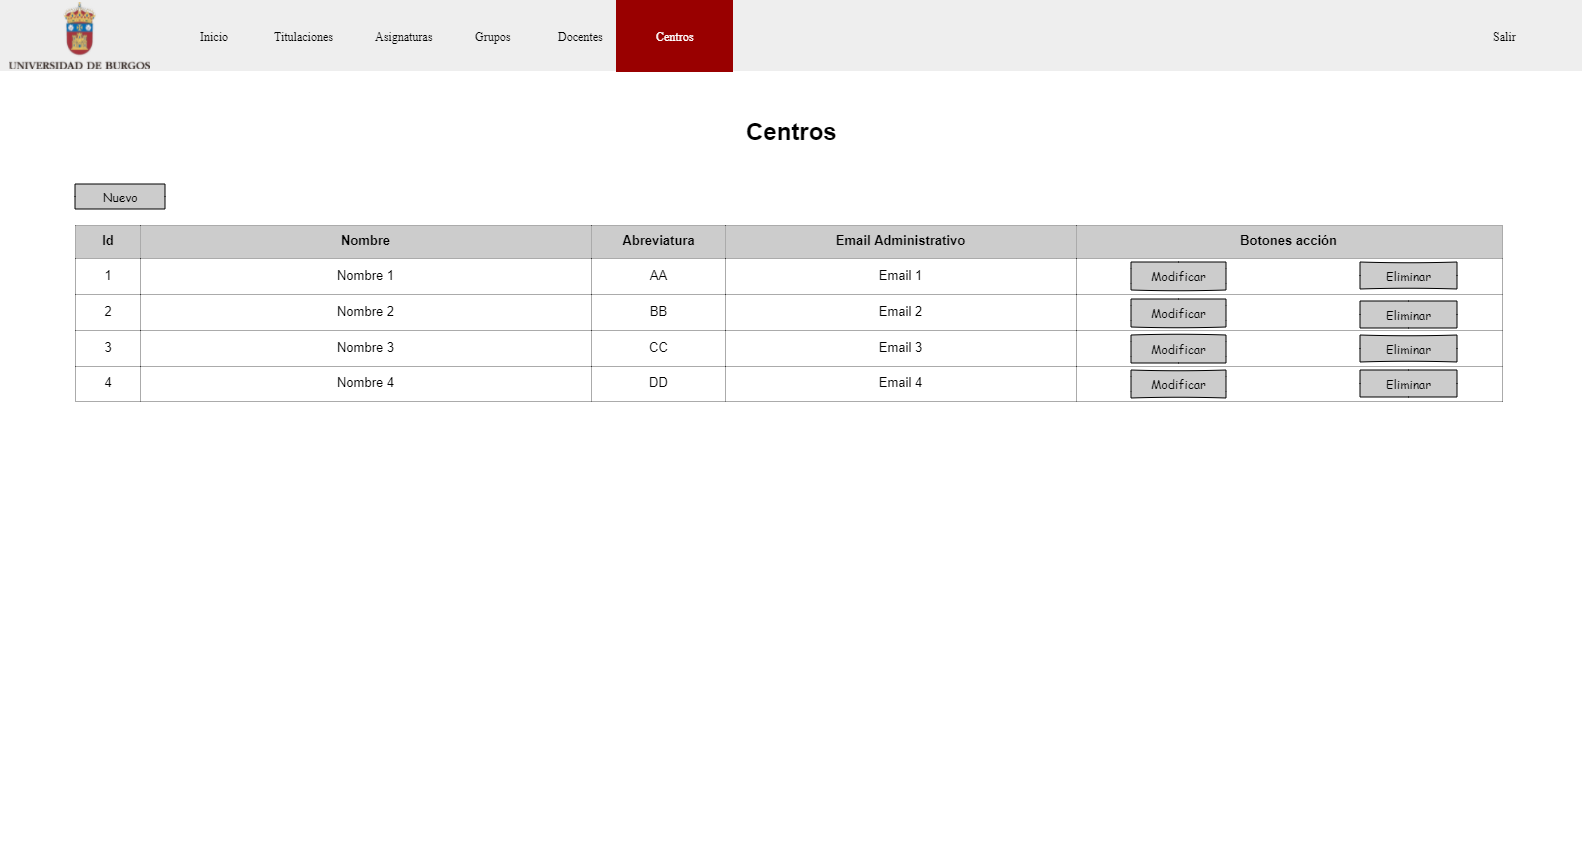
\includegraphics[width=\textwidth]{../img/Anexos/Vistas/centros.png}
		\caption{Mantenimiento de centros}
		\end{figure}
		\FloatBarrier
		\item \textbf{CU-1.1.1} Añadir/Modificar centros.
		\begin{figure}[!h]
		\centering
		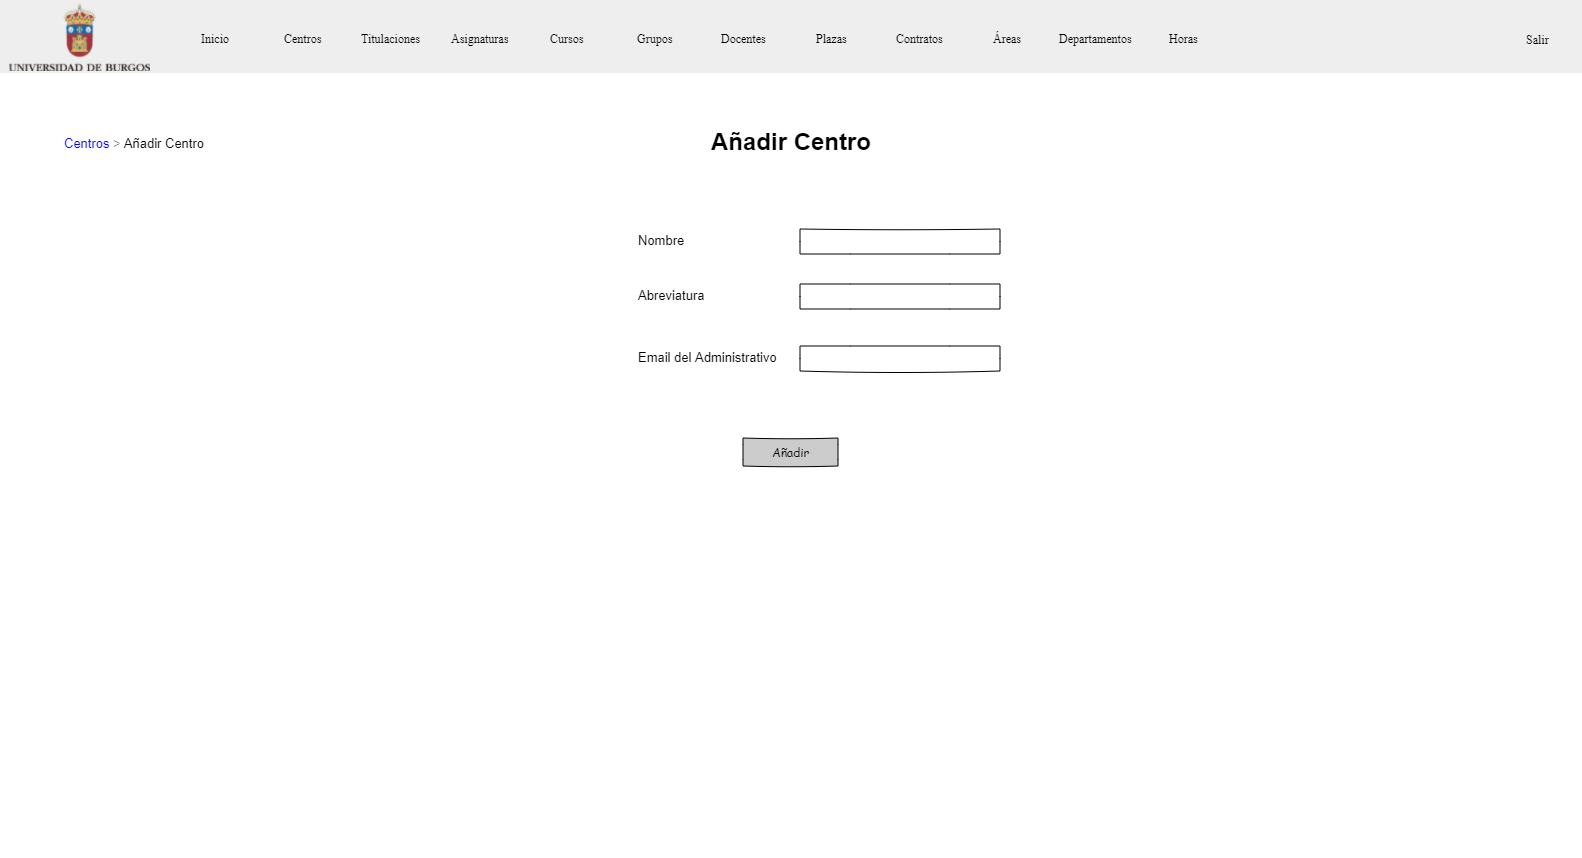
\includegraphics[width=\textwidth]{../img/Anexos/Vistas/add_centro.png}
		\caption{Añadir/Modificar centros}
		\end{figure}
		\FloatBarrier
		\item \textbf{CU-1.2} Mantenimiento de titulaciones.
		\begin{figure}[!h]
		\centering
		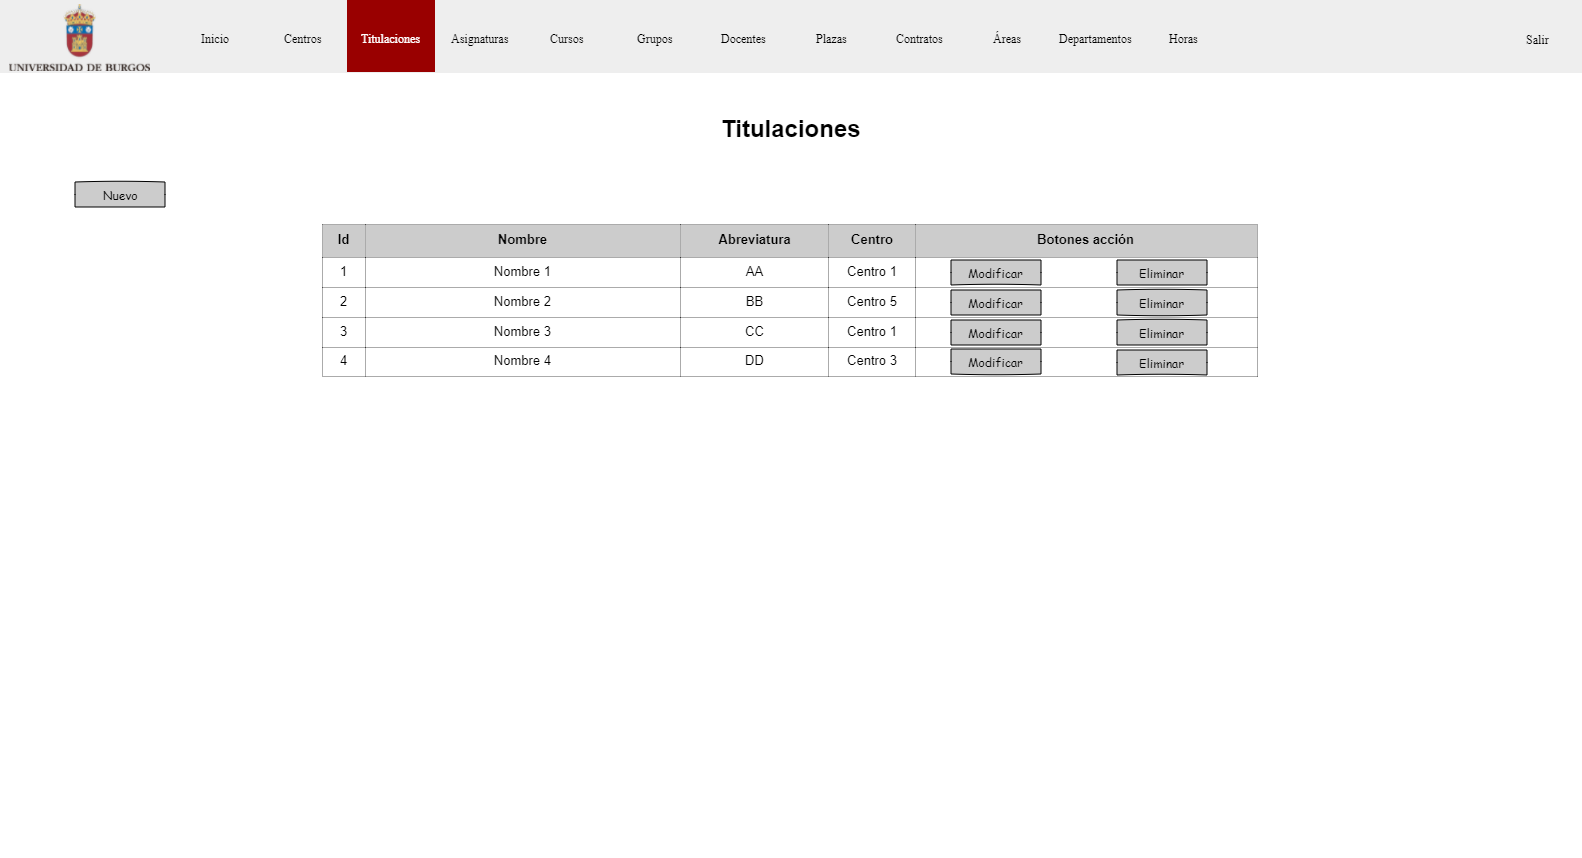
\includegraphics[width=\textwidth]{../img/Anexos/Vistas/titulaciones.png}
		\caption{Mantenimiento de titulaciones}
		\end{figure}
		\FloatBarrier
		\item \textbf{CU-1.2.1} Añadir/Modificar titulaciones.
		\begin{figure}[!h]
		\centering
		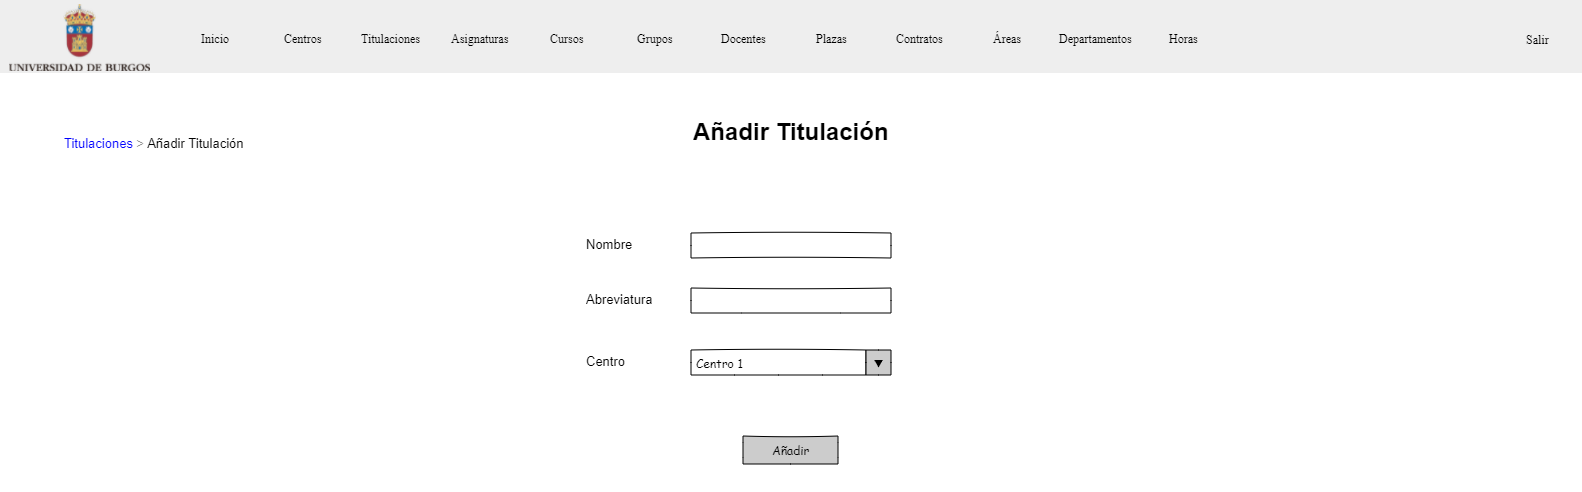
\includegraphics[width=\textwidth]{../img/Anexos/Vistas/add_titulacion.png}
		\caption{Añadir/Modificar titulaciones}
		\end{figure}
		\FloatBarrier
		\item \textbf{CU-1.3} Mantenimiento de asignaturas.
		\begin{figure}[!h]
		\centering
		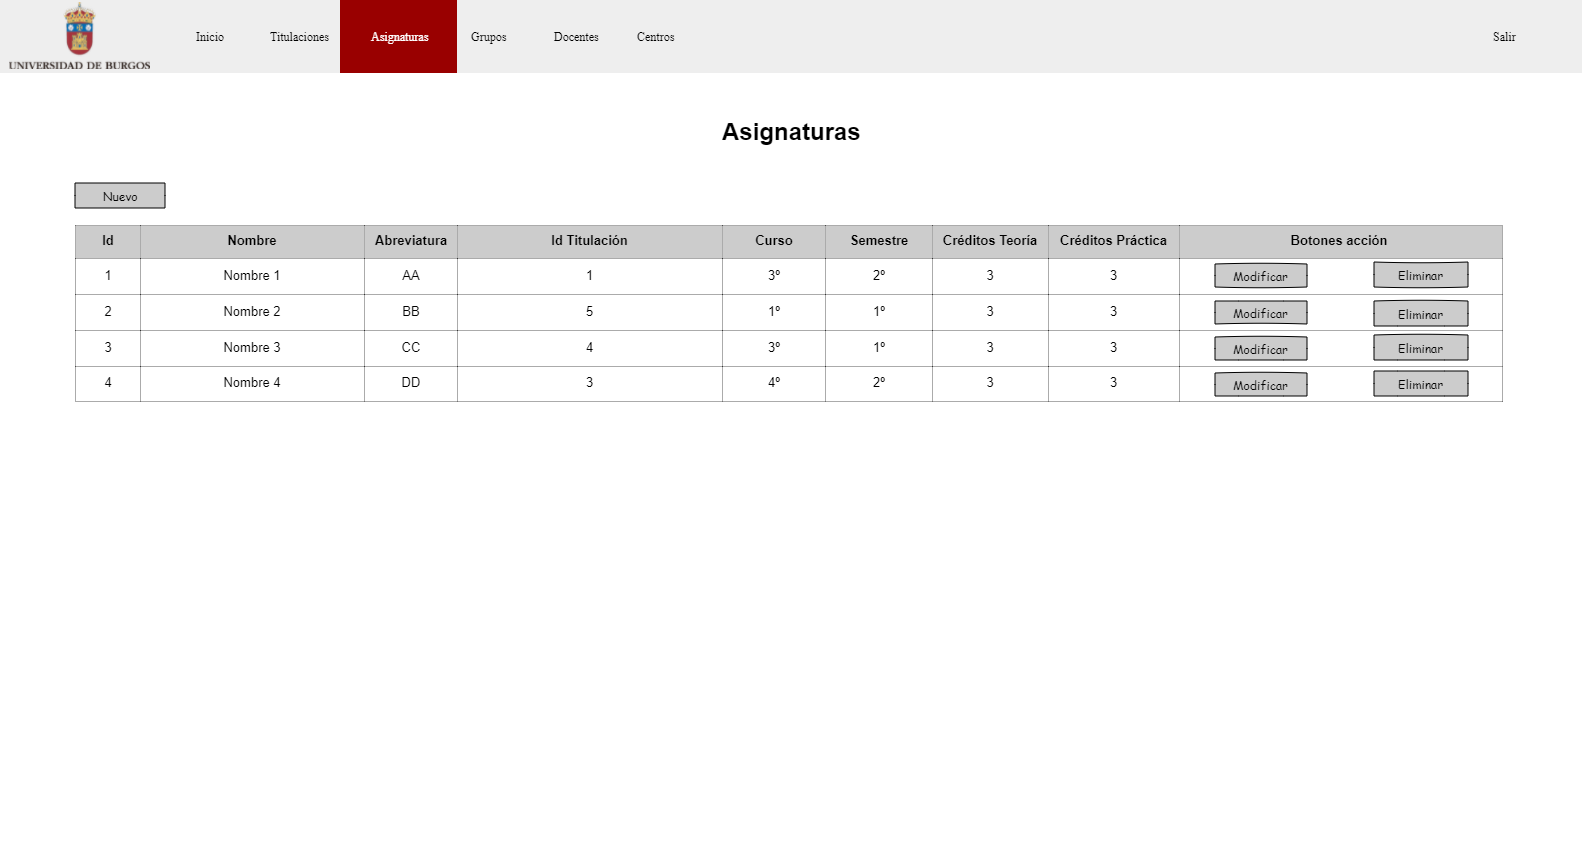
\includegraphics[width=\textwidth]{../img/Anexos/Vistas/asignaturas.png}
		\caption{Mantenimiento de asignaturas}
		\end{figure}
		\FloatBarrier
		\item \textbf{CU-1.3.1} Añadir/Modificar asignaturas.
		\begin{figure}[!h]
		\centering
		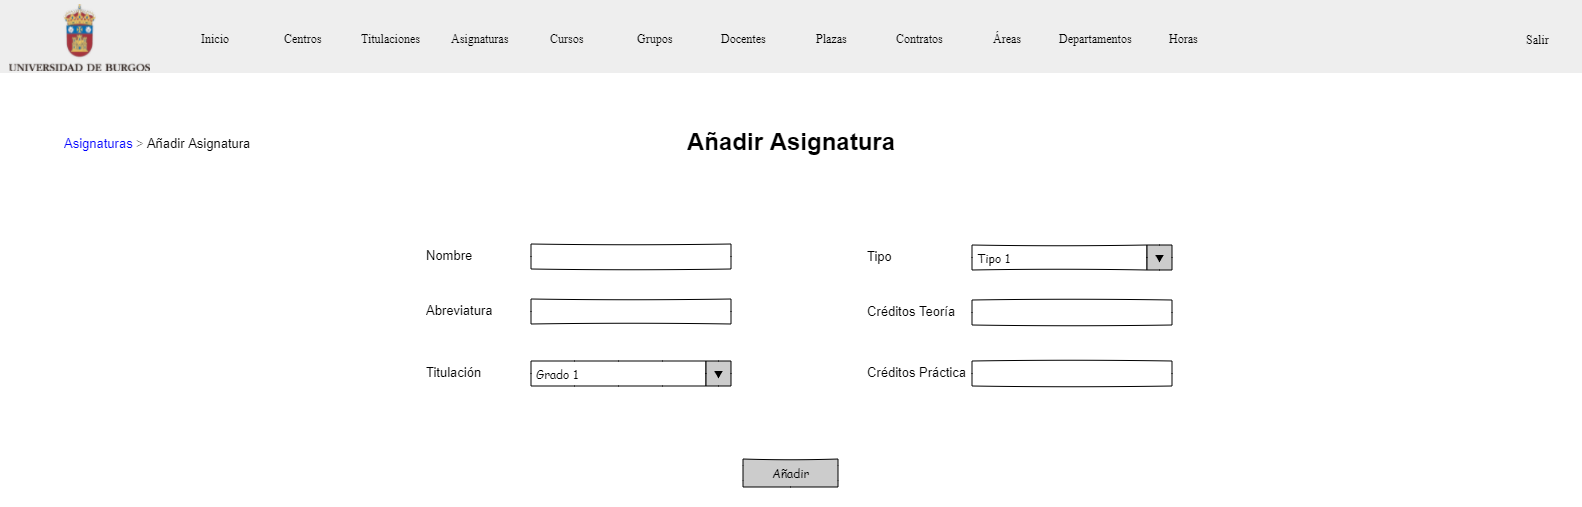
\includegraphics[width=\textwidth]{../img/Anexos/Vistas/add_asignatura.png}
		\caption{Añadir/Modificar asignaturas}
		\end{figure}
		\FloatBarrier
	\end{itemize}
	
	\item \textbf{CU-2.} Mantenimiento de profesorado.
	\begin{itemize}
		\item \textbf{CU-2.1} Mantenimiento de departamentos.
		\begin{figure}[!h]
		\centering
		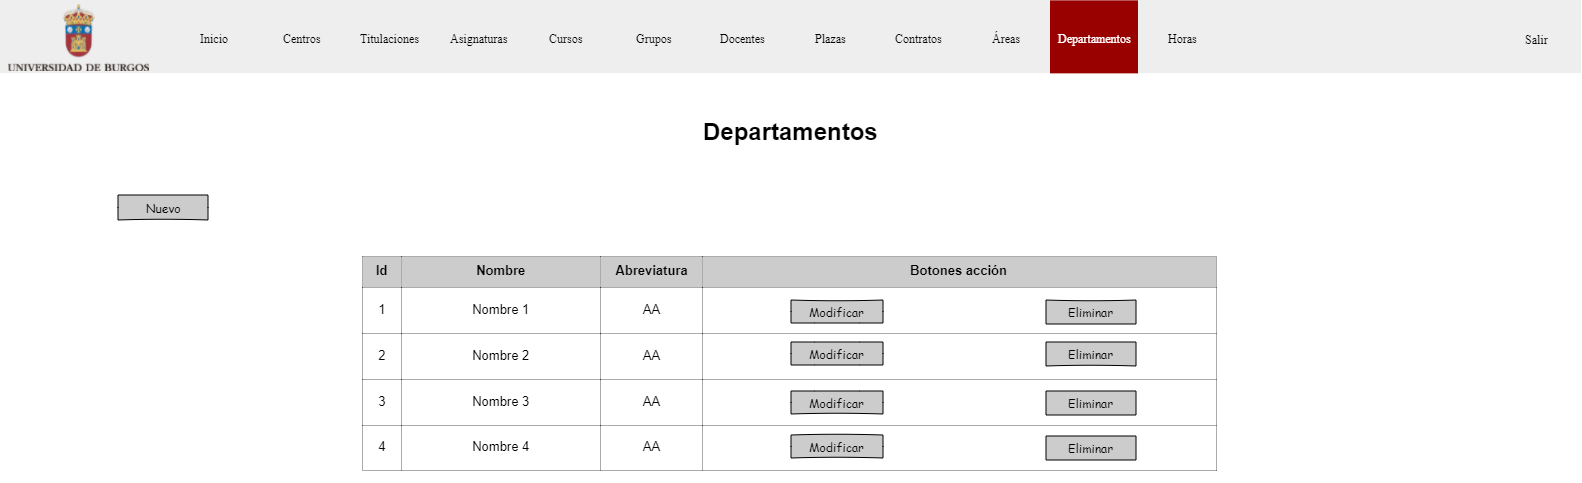
\includegraphics[width=\textwidth]{../img/Anexos/Vistas/departamentos.png}
		\caption{Mantenimiento de departamentos}
		\end{figure}
		\FloatBarrier
		\item \textbf{CU-2.1.1} Añadir/Modificar departamentos.
		\begin{figure}[!h]
		\centering
		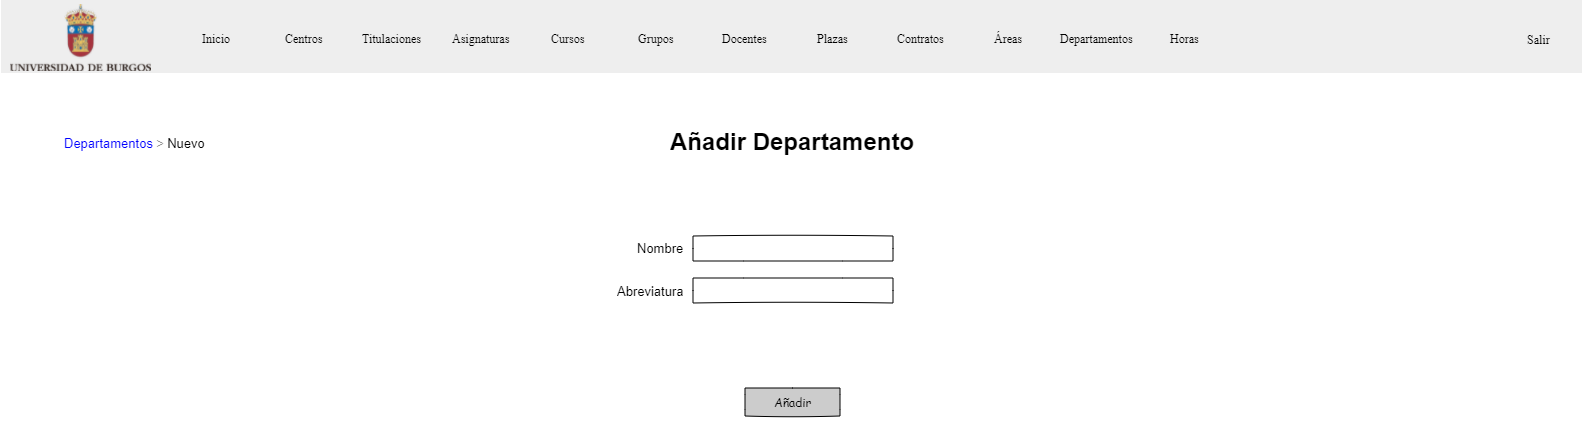
\includegraphics[width=\textwidth]{../img/Anexos/Vistas/add_departamento.png}
		\caption{Añadir/Modificar departamentos}
		\end{figure}
		\FloatBarrier
		\item \textbf{CU-2.2} Mantenimiento de áreas.
		\begin{figure}[!h]
		\centering
		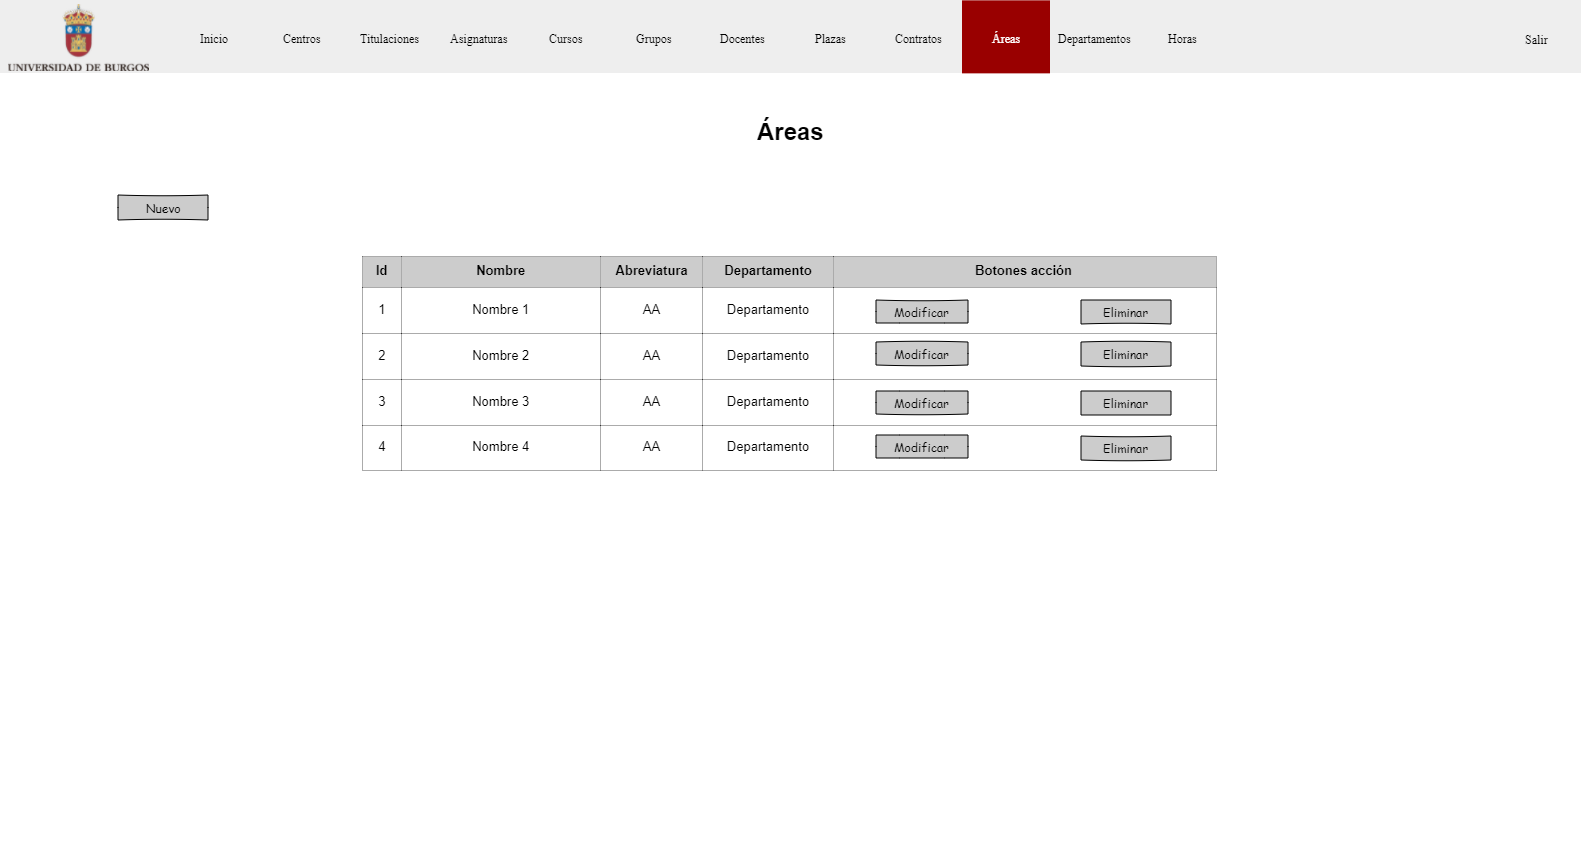
\includegraphics[width=\textwidth]{../img/Anexos/Vistas/areas.png}
		\caption{Mantenimiento de áreas}
		\end{figure}
		\FloatBarrier
		\item \textbf{CU-2.2.1} Añadir/Modificar áreas.
		\begin{figure}[!h]
		\centering
		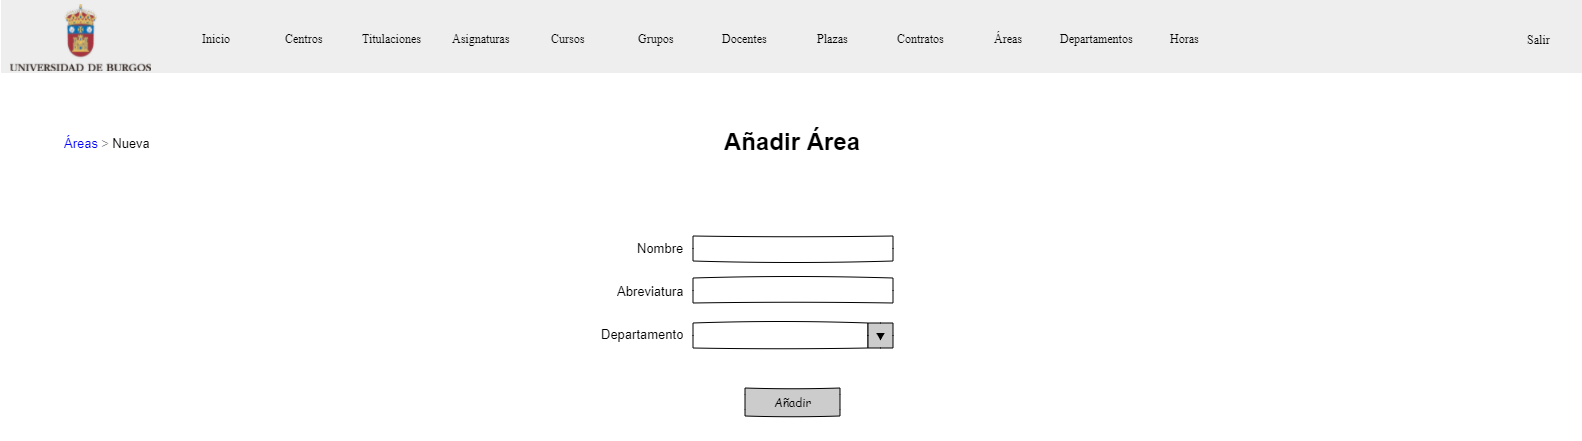
\includegraphics[width=\textwidth]{../img/Anexos/Vistas/add_area.png}
		\caption{Añadir/Modificar áreas}
		\end{figure}
		\FloatBarrier
		\item \textbf{CU-2.3} Mantenimiento de docentes.
		\begin{figure}[!h]
		\centering
		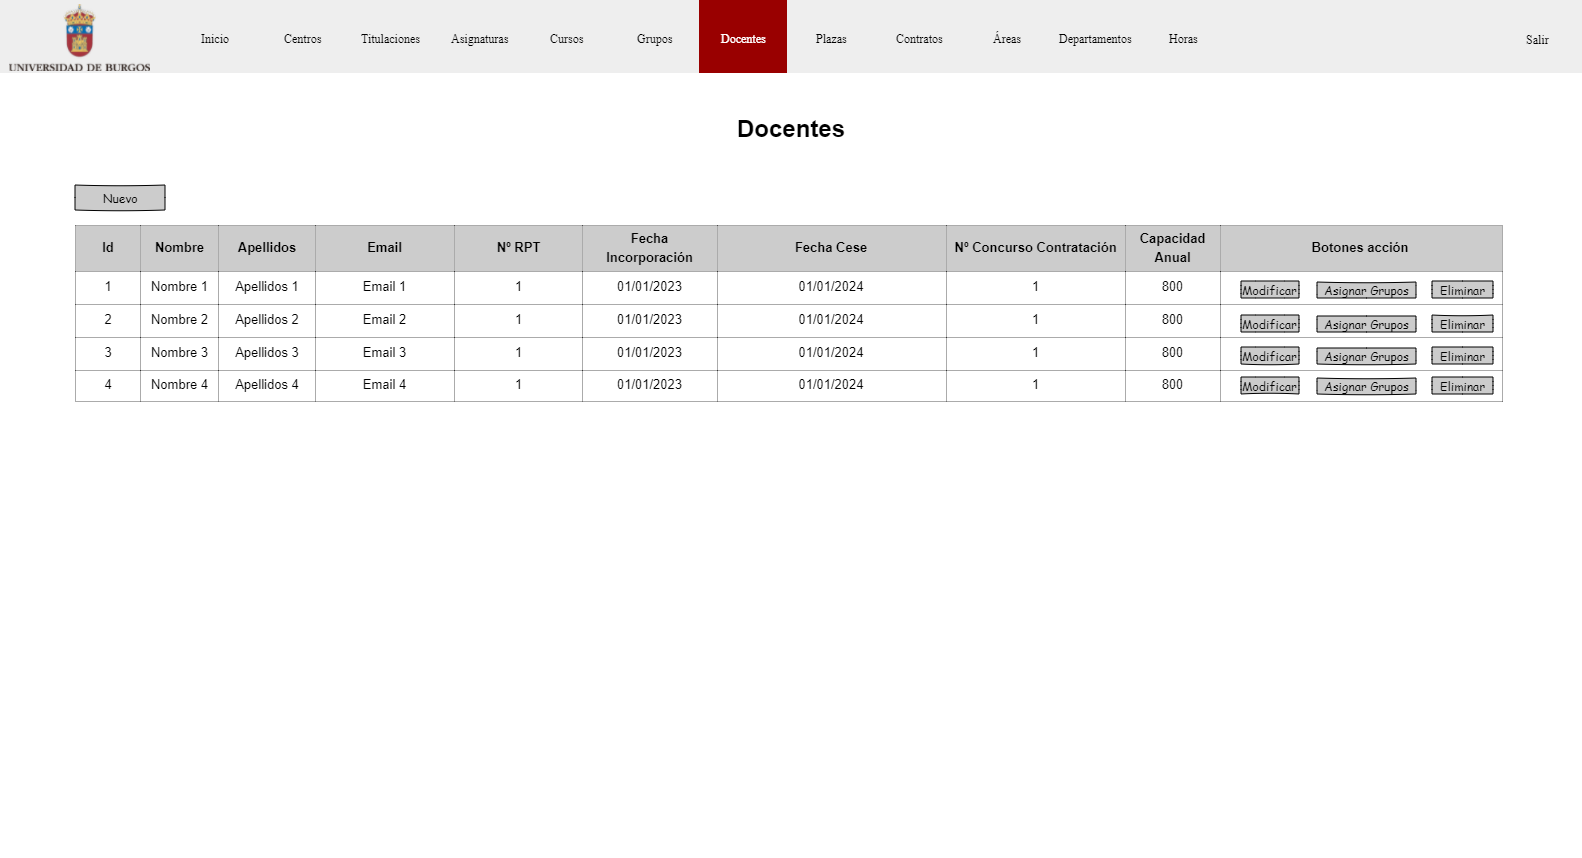
\includegraphics[width=\textwidth]{../img/Anexos/Vistas/docentes.png}
		\caption{Mantenimiento de docentes}
		\end{figure}
		\FloatBarrier
		\item \textbf{CU-2.3.1} Añadir/Modificar docentes.
		\begin{figure}[!h]
		\centering
		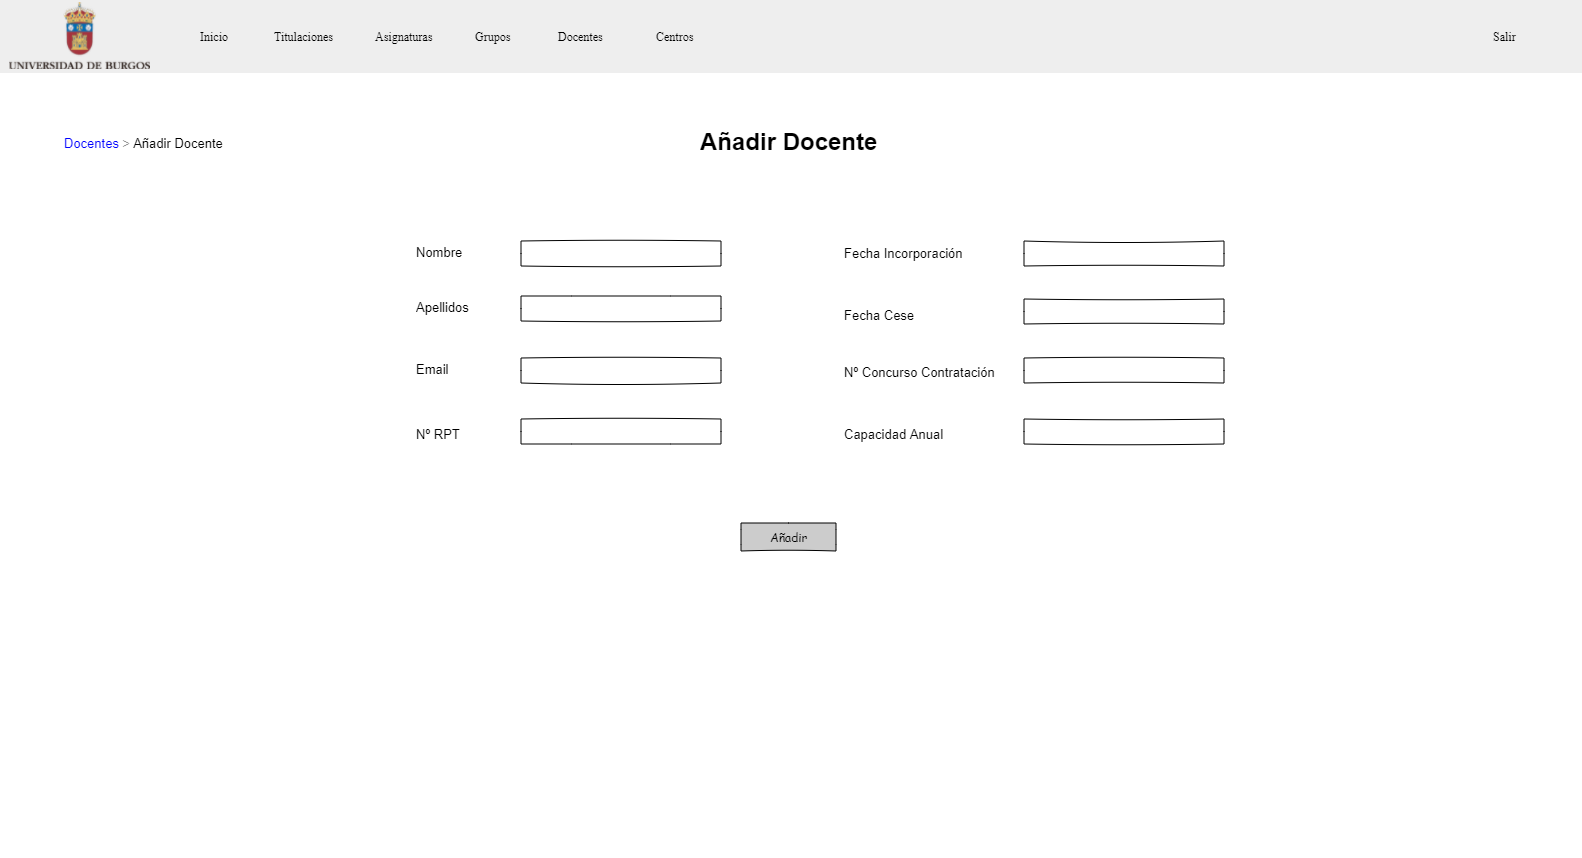
\includegraphics[width=\textwidth]{../img/Anexos/Vistas/add_docente.png}
		\caption{Añadir/Modificar docentes}
		\end{figure}
		\FloatBarrier
		\item \textbf{CU-2.4} Mantenimiento de tipos de contrato.
		\begin{figure}[!h]
		\centering
		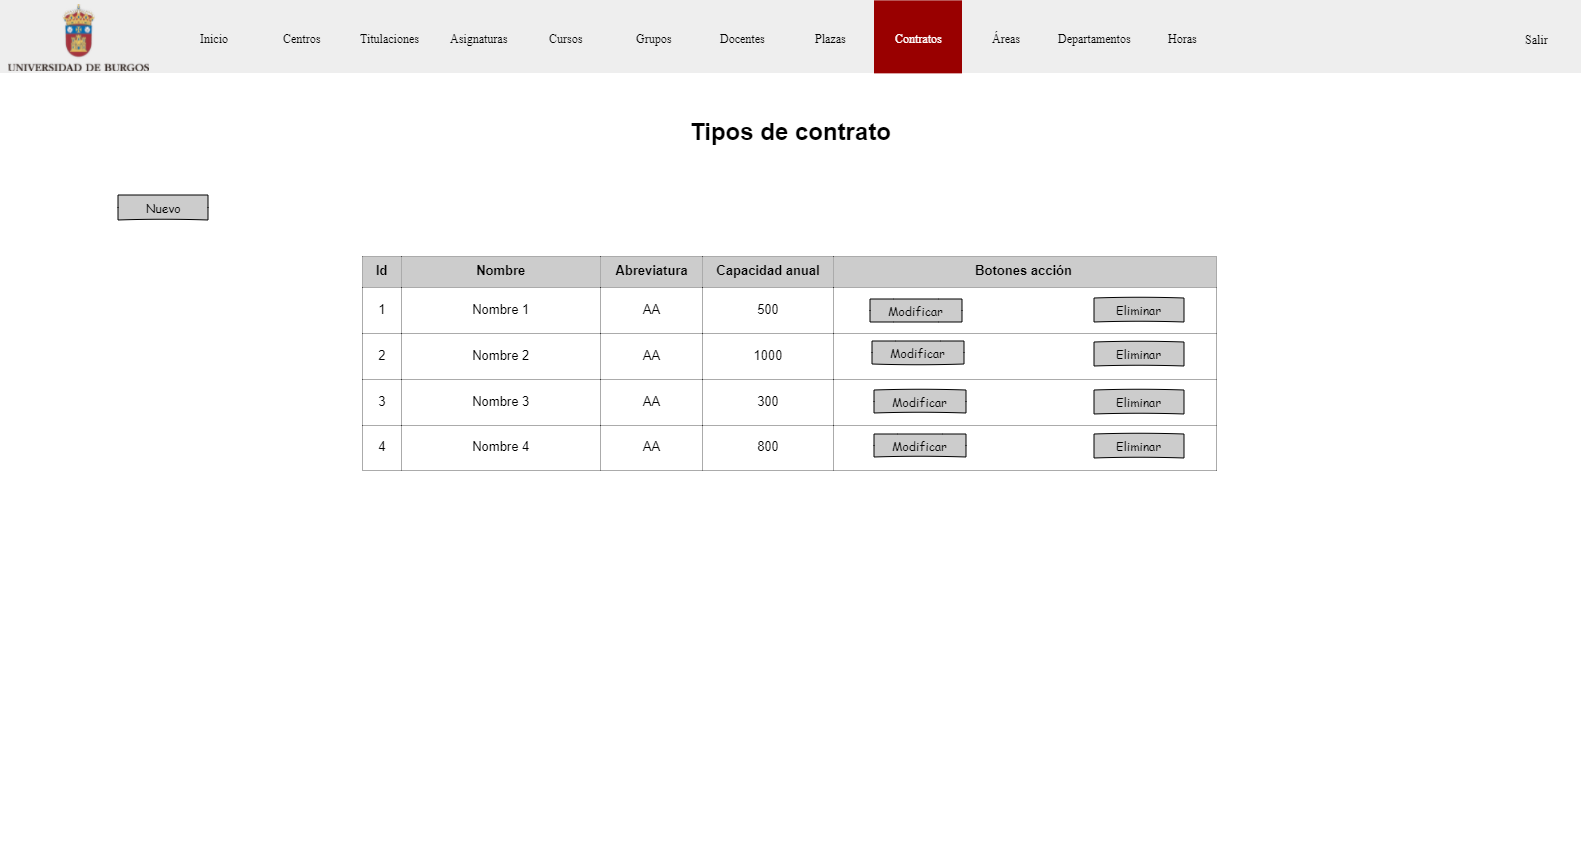
\includegraphics[width=\textwidth]{../img/Anexos/Vistas/contratos.png}
		\caption{Mantenimiento de tipos de contrato}
		\end{figure}
		\FloatBarrier
		\item \textbf{CU-2.4.1} Añadir/Modificar tipos de contrato.
		\begin{figure}[!h]
		\centering
		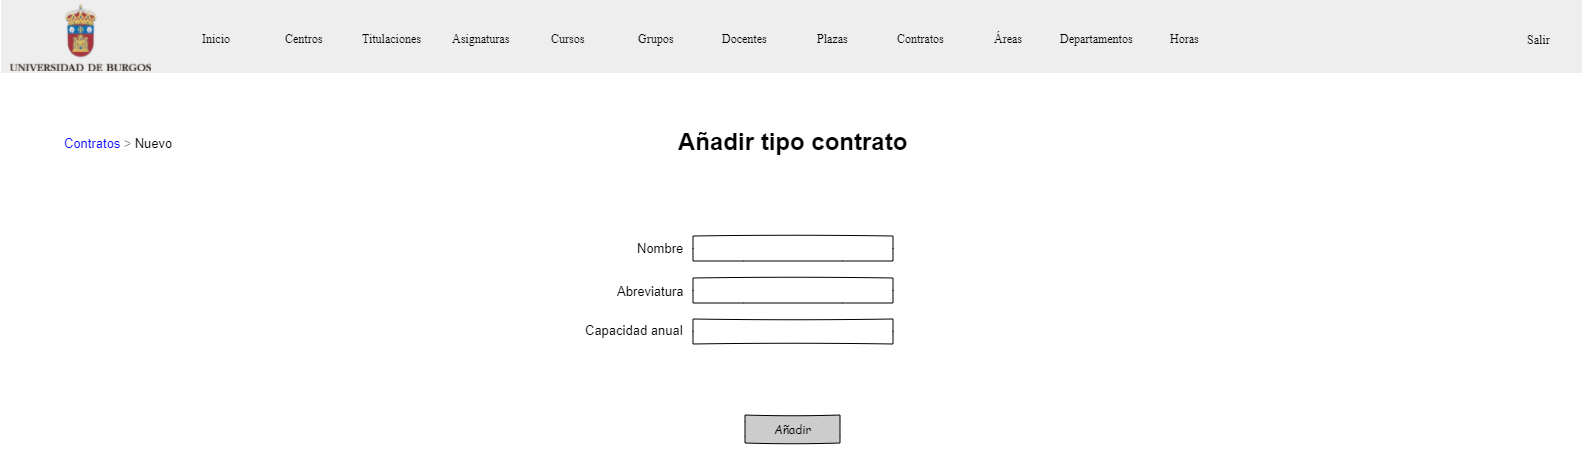
\includegraphics[width=\textwidth]{../img/Anexos/Vistas/add_contrato.png}
		\caption{Añadir/Modificar tipos de contrato}
		\end{figure}
		\FloatBarrier
		\item \textbf{CU-2.5} Mantenimiento de plazas.
		\begin{figure}[!h]
		\centering
		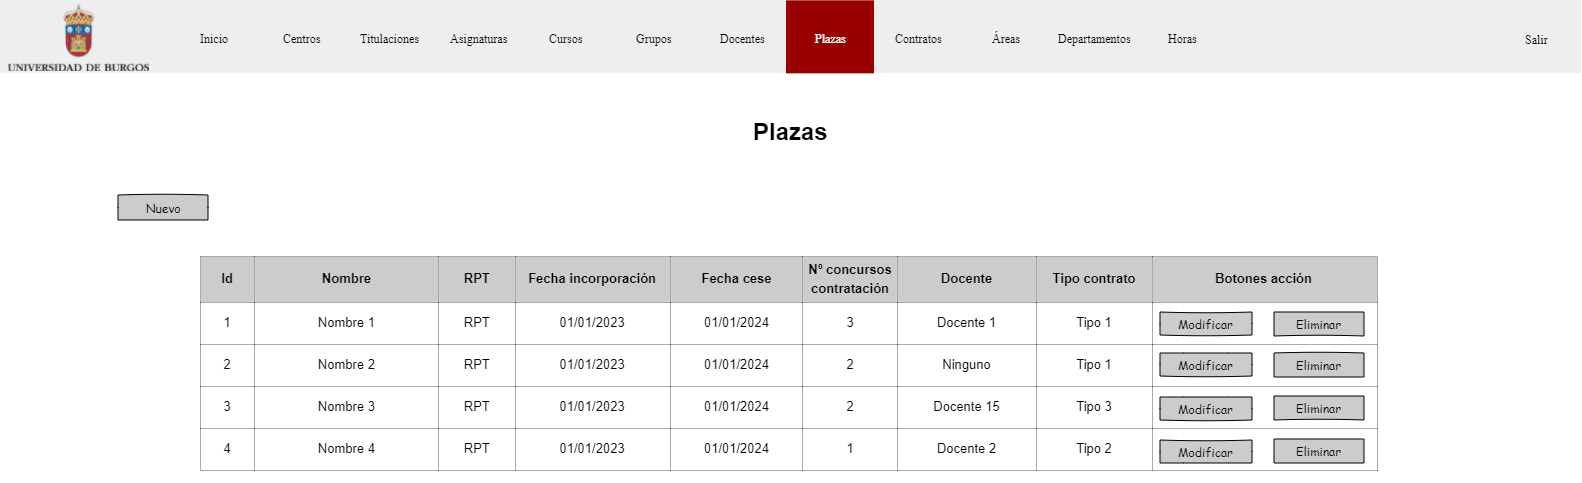
\includegraphics[width=\textwidth]{../img/Anexos/Vistas/plazas.png}
		\caption{Mantenimiento de plazas}
		\end{figure}
		\FloatBarrier
		\item \textbf{CU-2.5.1} Añadir/Modificar plazas.
		\begin{figure}[!h]
		\centering
		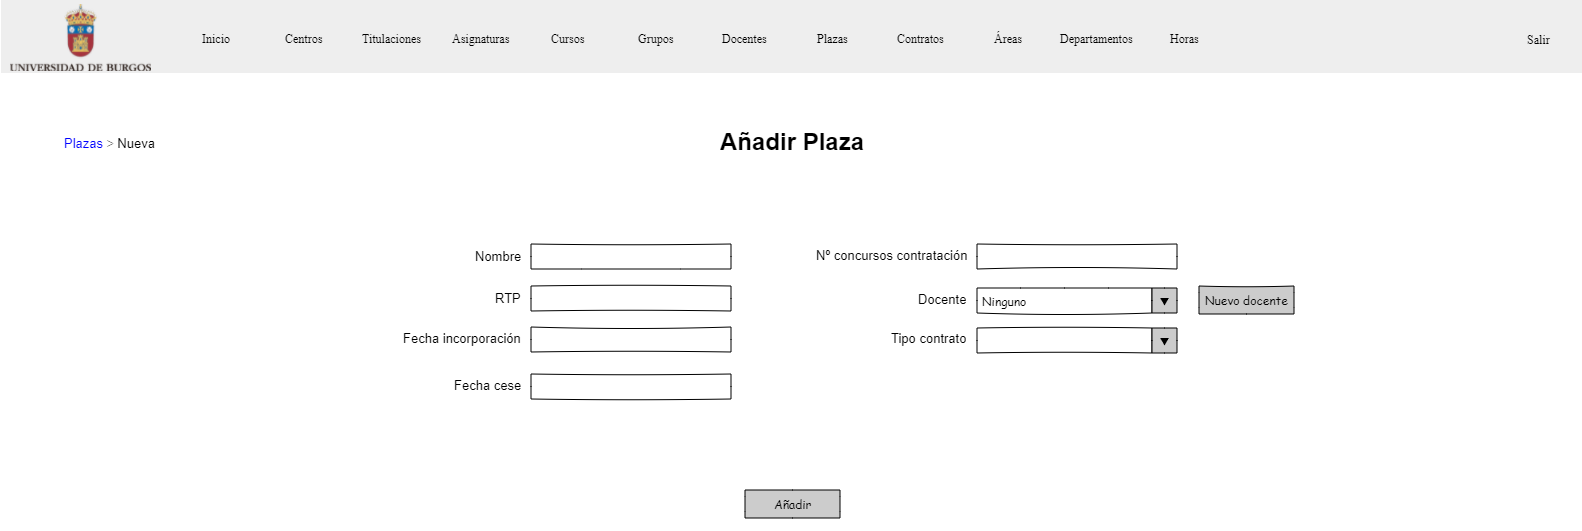
\includegraphics[width=\textwidth]{../img/Anexos/Vistas/add_plaza.png}
		\caption{Añadir/Modificar plazas}
		\end{figure}
		\FloatBarrier
		\item \textbf{CU-2.6} Asignar plaza a docente.
		\begin{figure}[!h]
		\centering
		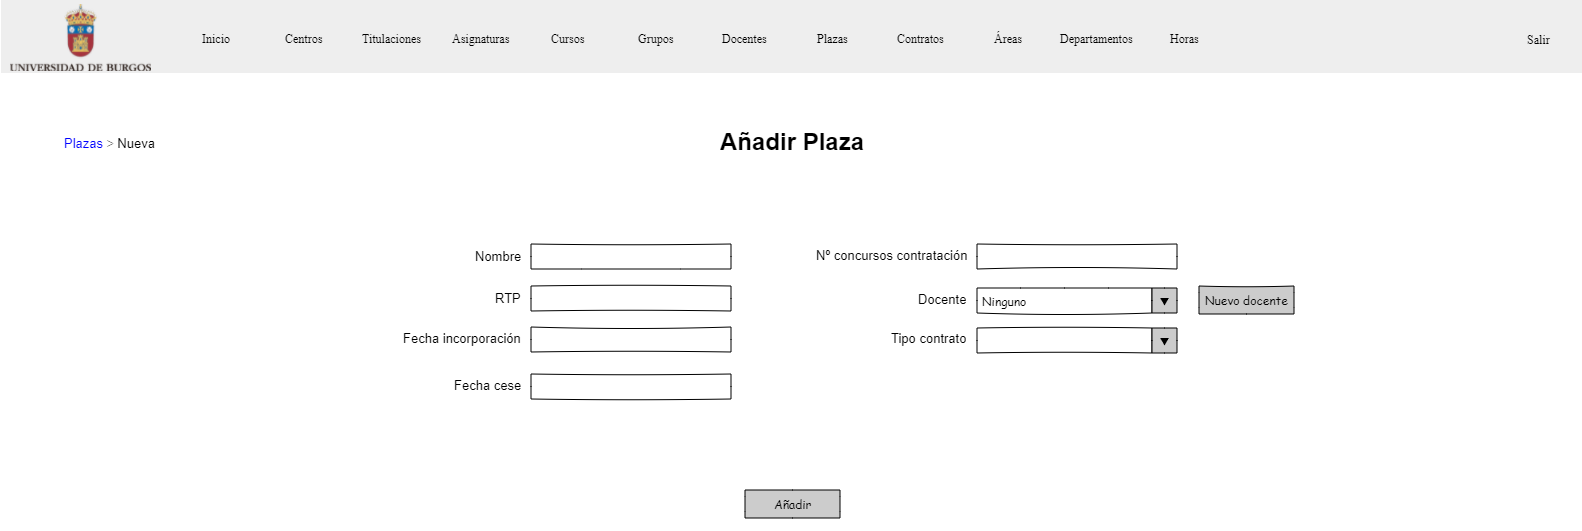
\includegraphics[width=\textwidth]{../img/Anexos/Vistas/add_plaza.png}
		\caption{Asignar plaza a docente}
		\end{figure}
		\FloatBarrier
	\end{itemize}
	
	\item \textbf{CU-3.} Asignación docente.
	\begin{itemize}
		\item \textbf{CU-3.1} Mantenimiento cursos académicos.
		\begin{figure}[!h]
		\centering
		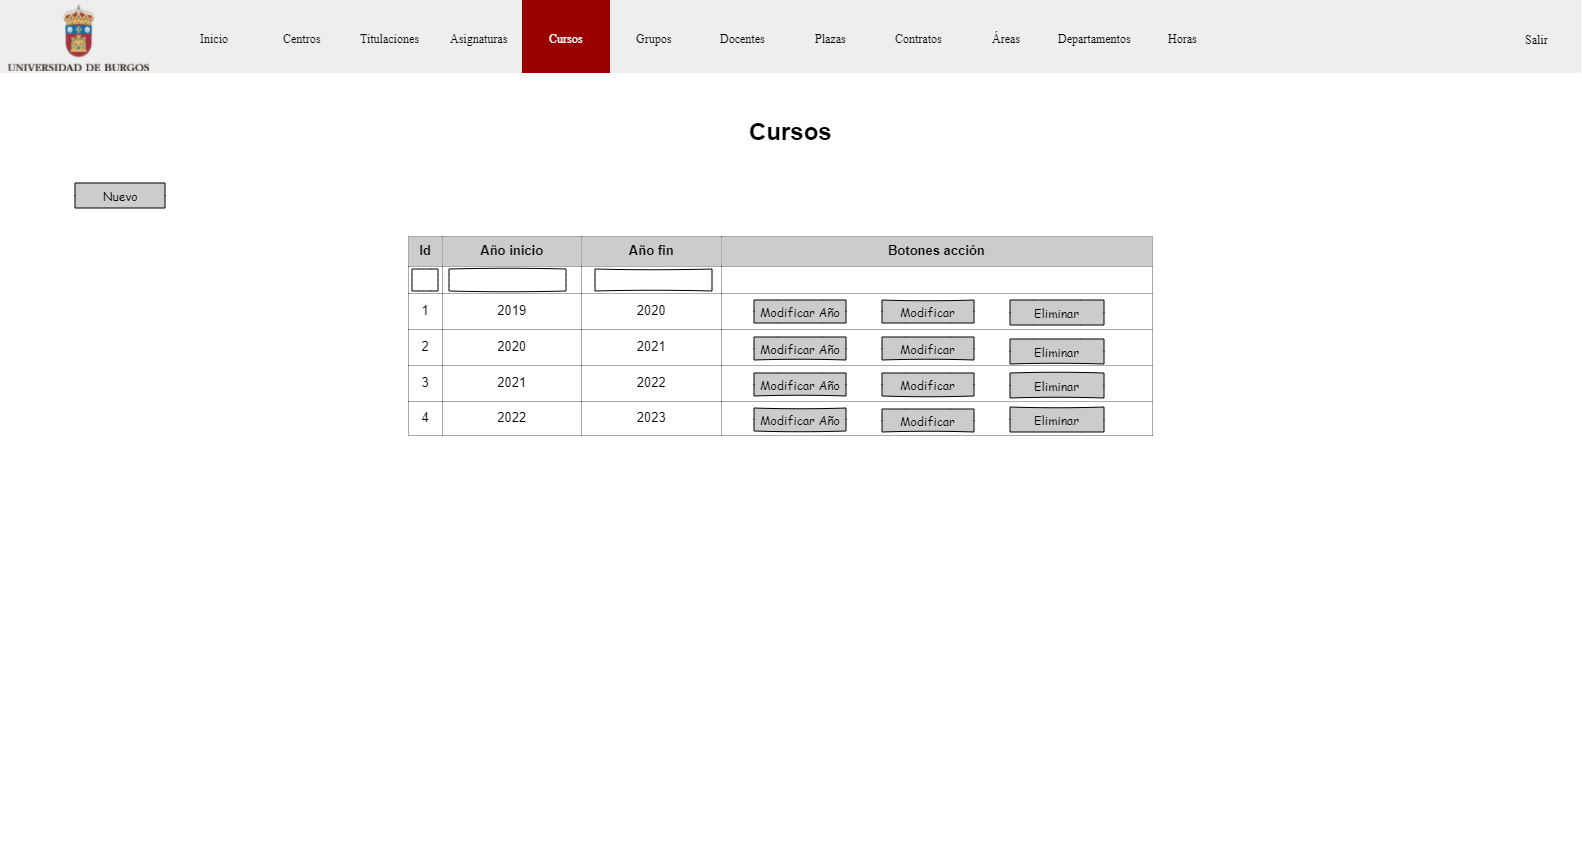
\includegraphics[width=\textwidth]{../img/Anexos/Vistas/cursos.png}
		\caption{Mantenimiento cursos académicos}
		\end{figure}
		\FloatBarrier
		\begin{figure}[!h]
		\centering
		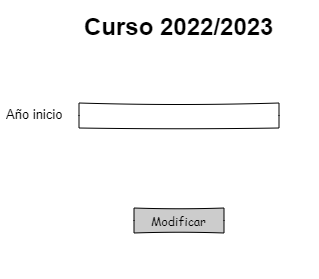
\includegraphics[width=0.7\textwidth]{../img/Anexos/Vistas/mod_ano_curso.png}
		\caption{Modificar año curso académico}
		\end{figure}
		\FloatBarrier
		\item \textbf{CU-3.1.1} Añadir curso académico.
		\begin{figure}[!h]
		\centering
		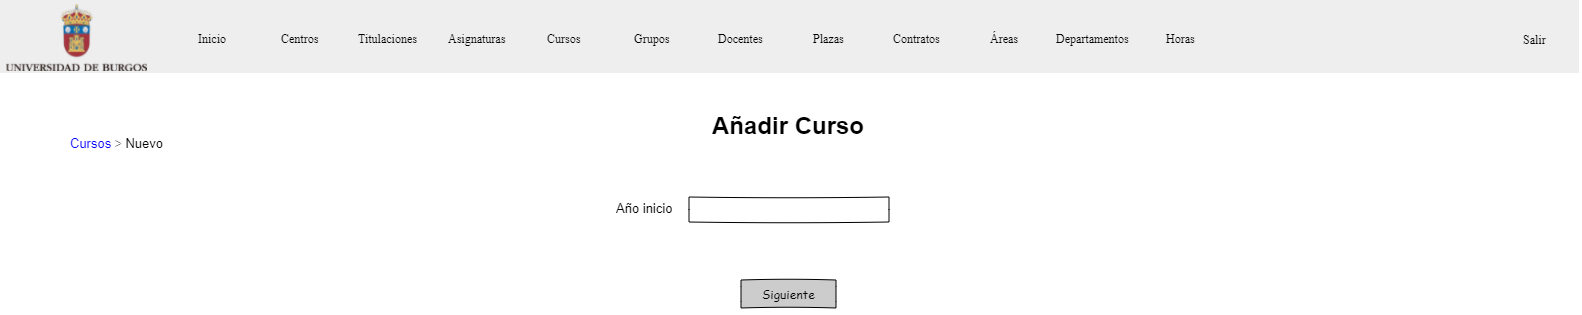
\includegraphics[width=\textwidth]{../img/Anexos/Vistas/add_curso.png}
		\caption{Añadir curso académico}
		\end{figure}
		\FloatBarrier
		\item \textbf{CU-3.1.2} Modificar curso académico.
		\begin{figure}[!h]
		\centering
		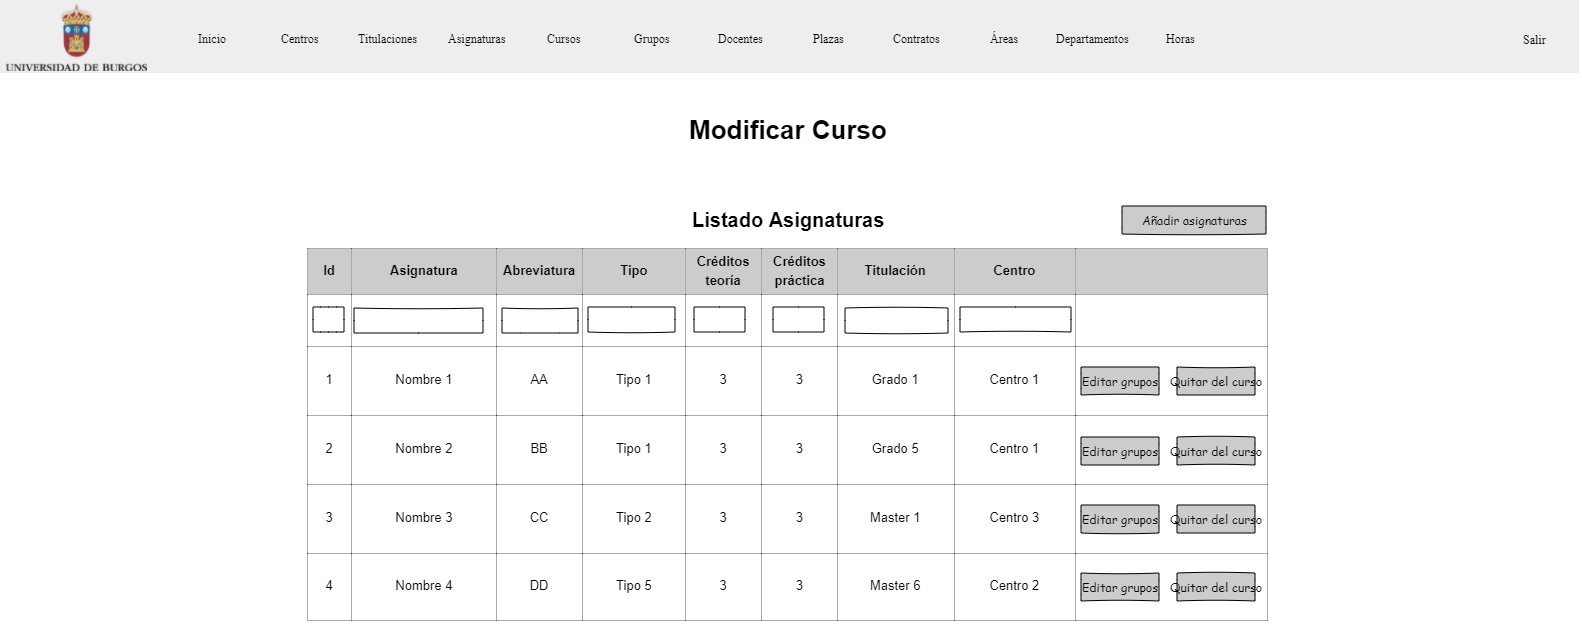
\includegraphics[width=\textwidth]{../img/Anexos/Vistas/mod_curso.png}
		\caption{Modificar curso académico}
		\end{figure}
		\FloatBarrier
		\begin{figure}[!h]
		\centering
		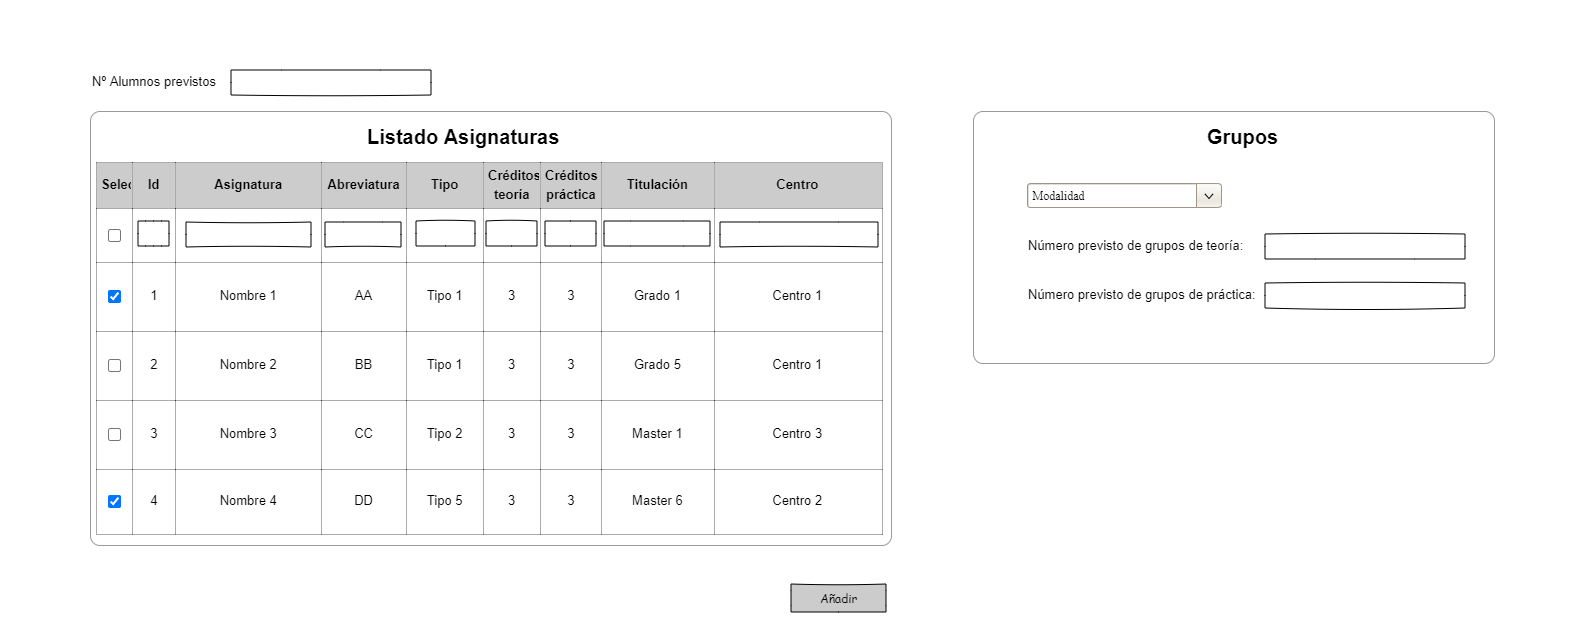
\includegraphics[width=\textwidth]{../img/Anexos/Vistas/add_asig.png}
		\caption{Añadir asignaturas al curso}
		\end{figure}
		\FloatBarrier
		\item \textbf{CU-3.2} Mantenimiento de grupos.
		\begin{figure}[!h]
		\centering
		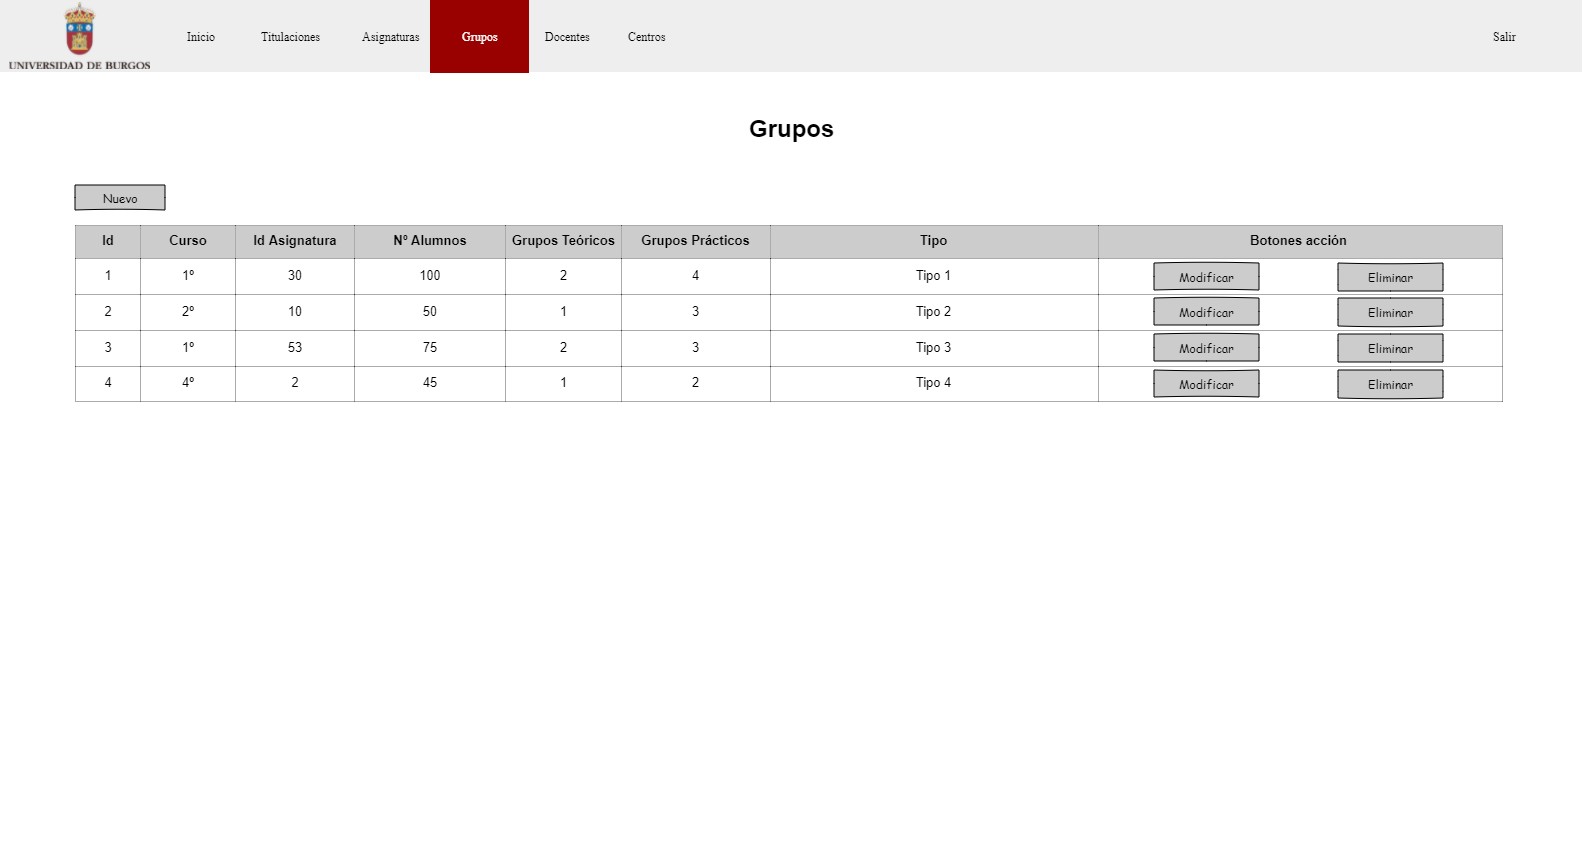
\includegraphics[width=\textwidth]{../img/Anexos/Vistas/grupos.png}
		\caption{Mantenimiento de grupos}
		\end{figure}
		\FloatBarrier
		\item \textbf{CU-3.2.1} Añadir/Modificar grupo.
		\begin{figure}[!h]
		\centering
		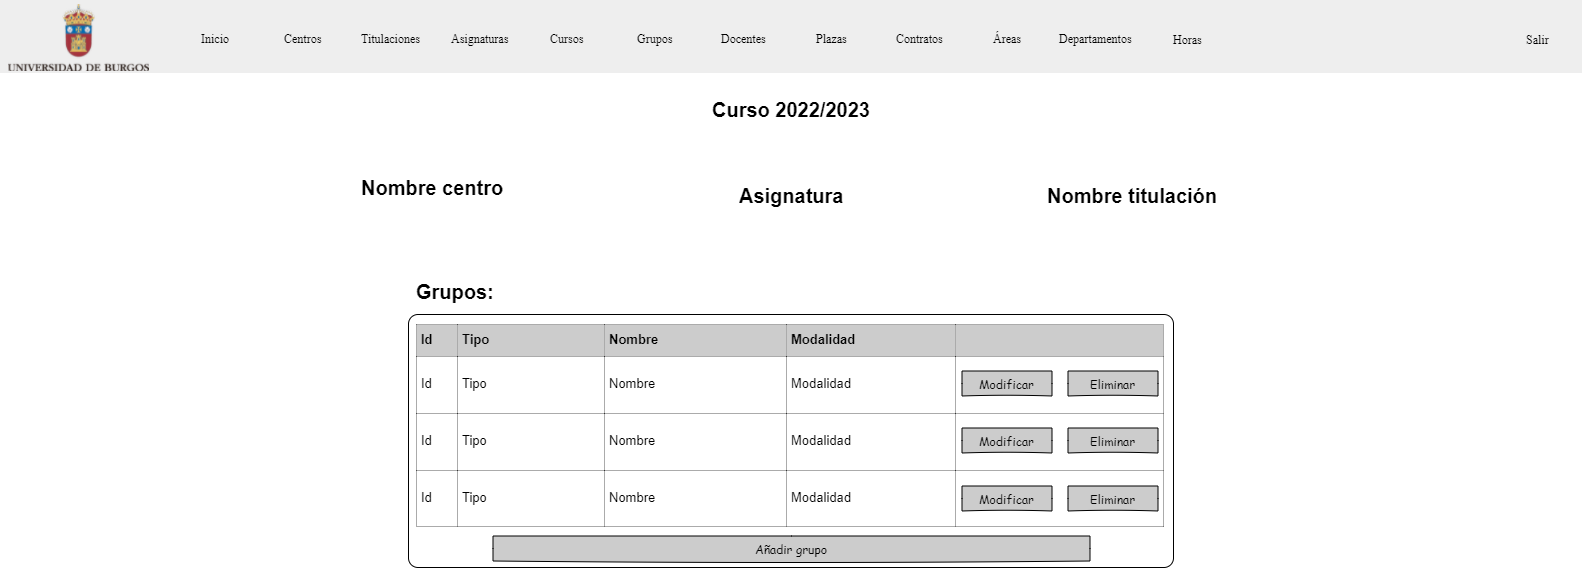
\includegraphics[width=\textwidth]{../img/Anexos/Vistas/addmod_grupo.png}
		\caption{Añadir/Modificar grupo}
		\end{figure}
		\FloatBarrier
		\begin{figure}[!h]
		\centering
		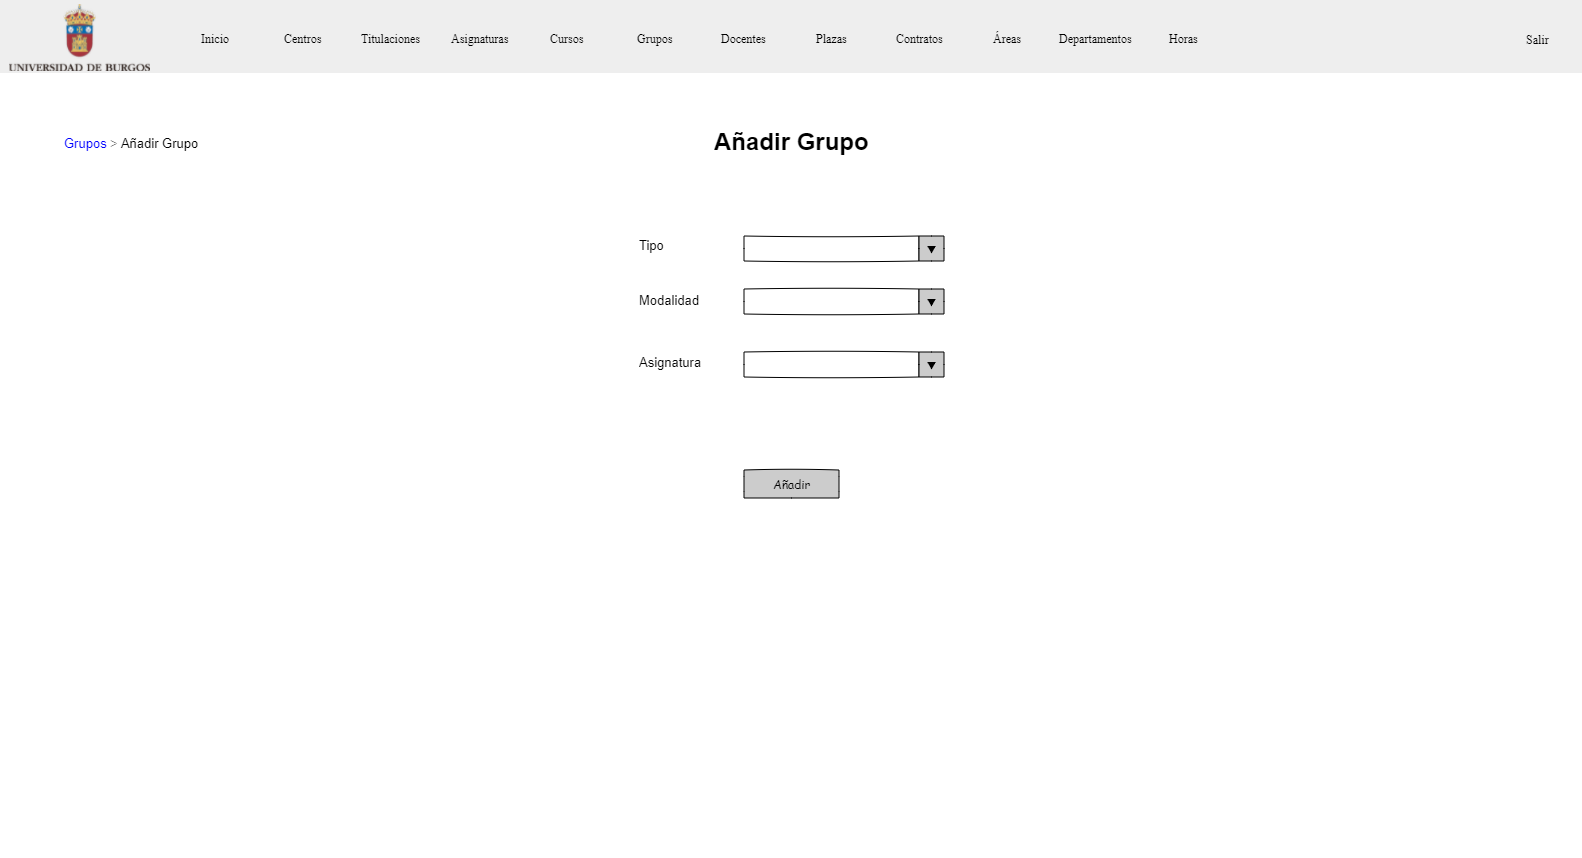
\includegraphics[width=0.7\textwidth]{../img/Anexos/Vistas/add_grupo.png}
		\caption{Añadir/Modificar grupo 2}
		\end{figure}
		\FloatBarrier
		\item \textbf{CU-3.3} Asignación de horas de plazas a grupos.
		\begin{figure}[!h]
		\centering
		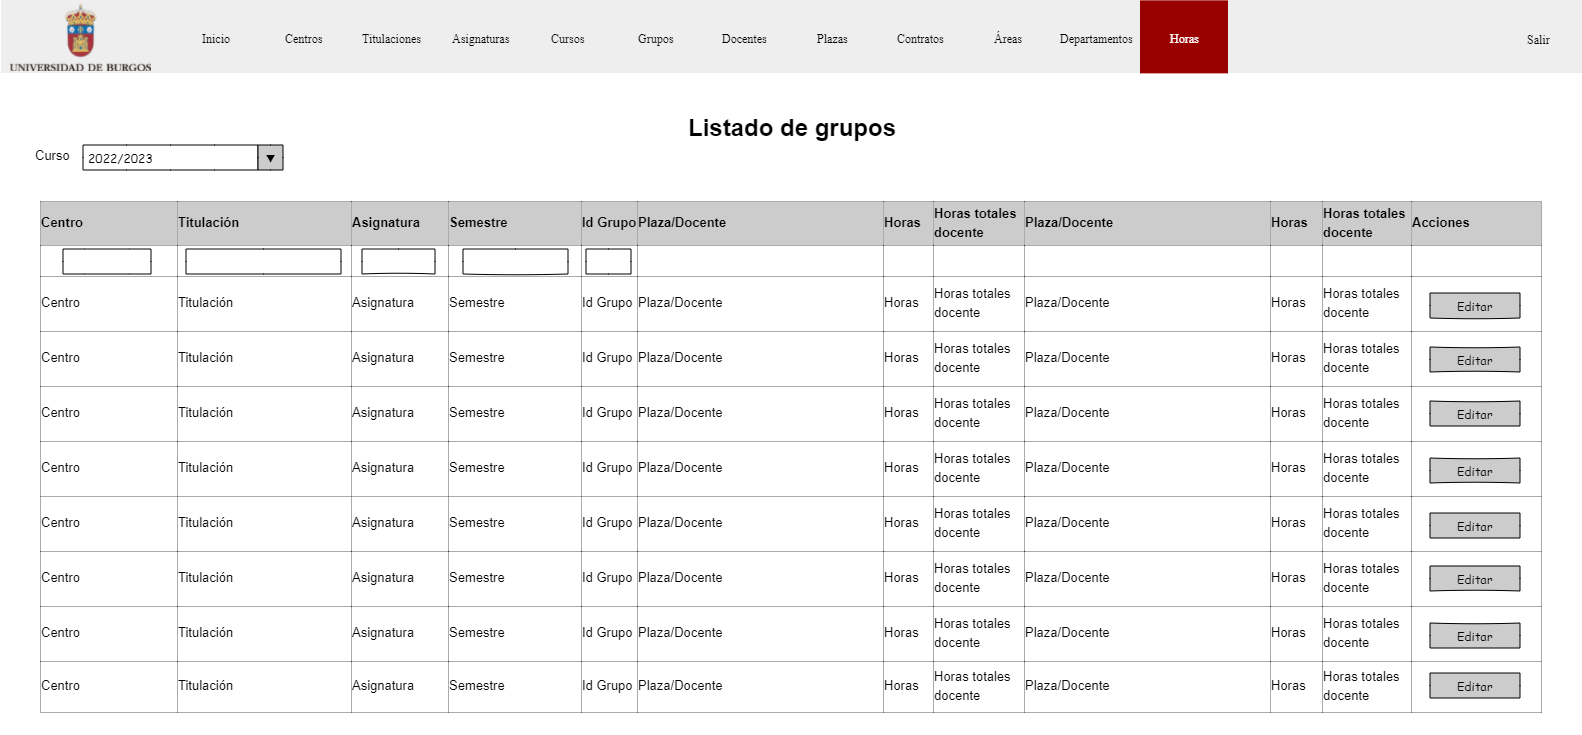
\includegraphics[width=\textwidth]{../img/Anexos/Vistas/horas.png}
		\caption{Asignación de horas de plazas a grupos}
		\end{figure}
		\FloatBarrier
		\begin{figure}[!h]
		\centering
		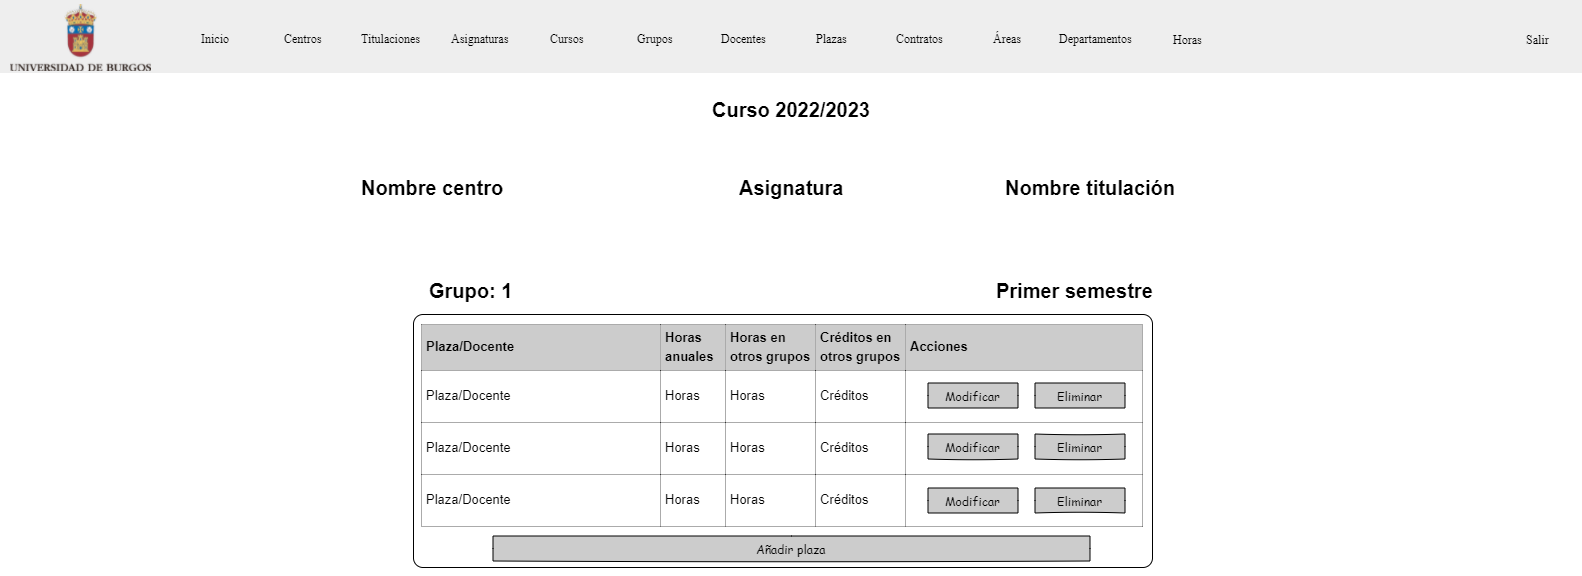
\includegraphics[width=\textwidth]{../img/Anexos/Vistas/asig_horas_plaza_grupo.png}
		\caption{Asignación de horas de plazas a grupos 2}
		\end{figure}
		\FloatBarrier
		\begin{figure}[!h]
		\centering
		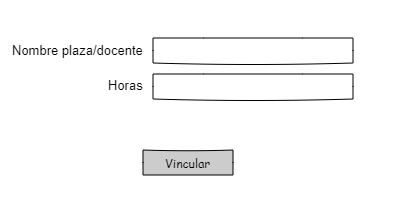
\includegraphics[width=0.7\textwidth]{../img/Anexos/Vistas/asig_horas_plaza_grupo_modal.png}
		\caption{Asignación de horas de plazas a grupos 3}
		\end{figure}
		\FloatBarrier
	\end{itemize}
\end{itemize}


